\documentclass[titlepage, 11pt]{article}
\usepackage[a4paper, total={6in, 9.5in}]{geometry}
\usepackage{graphicx}
\usepackage{advdate}
\usepackage{amsmath,amsfonts,amssymb}
\usepackage{listings}
\usepackage{booktabs}
\usepackage[T1]{fontenc}
\usepackage{listings}
\usepackage{color}
\usepackage{xspace}
\usepackage{minted}
\usepackage[colorlinks=true, linkcolor=blue, urlcolor=blue, citecolor=blue, pdfborder={0 0 255}]{hyperref}
\usepackage{colortbl}
\usepackage{url}
\usepackage{xcolor}
\usepackage{caption}
\usepackage{subcaption}
\usepackage{dirtytalk}
\usepackage[semicolon, round]{natbib}
\usepackage[ruled]{algorithm2e}
\captionsetup[table]{skip=10pt}
\renewcommand{\vec}[1]{\mathbf{#1}}
\SetKwComment{Comment}{$\triangleright$\ }{}
% \hypersetup{%
% 	colorlinks=true,
% 	linkcolor=blue,
% 	linkbordercolor={0 0 1}
% }

% \renewcommand\lstlistingname{Algorithm}
% \renewcommand\lstlistlistingname{Algorithms}
% \def\lstlistingautorefname{Alg.}

% \lstdefinestyle{Python}{
% 	language        = Python,
% 	frame           = lines, 
% 	basicstyle      = \footnotesize,
% 	keywordstyle    = \color{blue},
% 	stringstyle     = \color{green},
% 	commentstyle    = \color{red}\ttfamily
% }

% \setlength{\parindent}{0.0in}
% \setlength{\parskip}{0.05in}

\newcommand{\argmin}{\mathop{\mathrm{argmin}}}
\newcommand{\argmax}{\mathop{\mathrm{argmax}}}
\newcommand{\minimize}{\mathop{\mathrm{minimize}}}
\newcommand{\maximize}{\mathop{\mathrm{maximize}}}
\newcommand{\st}{\mathop{\mathrm{subject\,\,to}}}
\newcommand{\dist}{\mathop{\mathrm{dist}}}
\newcommand{\norm}[1]{\left\lVert#1\right\rVert}
\renewcommand{\vec}[1]{\mathbf{#1}}

\def\R{\mathbb{R}}
\def\E{\mathbb{E}}
\def\P{\mathbb{P}}
\def\S{\mathbb{S}}
\def\Cov{\mathrm{Cov}}
\def\Var{\mathrm{Var}}
\def\half{\frac{1}{2}}
\def\quat{\frac{1}{4}}
\def\sign{\mathrm{sign}}
\def\supp{\mathrm{supp}}
\def\th{\mathrm{th}}
\def\tr{\mathrm{tr}}
\def\dim{\mathrm{dim}}
\def\dom{\mathrm{dom}}

\title{
{EE1103: Numerical Methods} \\~\\
{\vlarge Programming Assignment {\#} 1}\\
}\author{ANIRUDH B S, EE21B019\\
Collaborators: & AMIZHTHNI P R K, EE21B015
 & ANKITA HARSHA MURTHY, EE21B020}
\date{\today}

\begin{document}
\maketitle
\setcounter{page}{0}
\tableofcontents
\listoffigures
\listoftables
\newpage

\section{Problem 1}
Determine the positive real root 
\begin{align}
    f(x) = \ln{x^4} - 0.7
\end{align} 

\begin{itemize}
    \item [(a)]  Plot the function by choosing a reasonable range for x to understand the nature of the function.
    
    \item [(b)] Find its root using three iterations of the bisection method, with initial guesses of $x_l$ = 0.5 and $x_u$ = 2, and .
    
    \item [(c)] Use three iterations of the false-position method, with the same initial guesses as in (b) and find the root.
 
    \item [(d)] Summarize your results in a table - against each iteration, record the approximate value and approximate error in both the methods.
\end{itemize}

\subsection{Approach}

We solve the given problem using both the methods listed below. 
\begin{itemize}
    \item [(1)] Bisection Method
    \item [(2)] False Position Method
\end{itemize}

In this problem, we use iterative procedure to find the root. Both Bisection Method and False Position are considered as Bracketing Methods as we divide the original interval into two sub-intervals and search for the root in the respective interval. 

%%%%%%%%%%%%%%%%%%%%%%%%%%%%%%%%%%%%%%%%%%%%%%%%%%%%%%

\subsection{Algorithm}
In this section, I present the pseudocode/flowchart of the algorithm used to solve the problem.

The pseudocode for finding the roots of f(x)=0 is provided in Algorithm~\ref{alg1} and Algorithm~\ref{alg2}.
\begin{center}
\begin{algorithm}[H]\label{alg1}

\SetAlgoLined

Input $x_l,x_u,x_r$ \\
ITER_{MAX} \gets 3 \\
count = 1 \\
\While{count<=ITER_{MAX}}{
$x_{rold} \gets x_r$ \;
$x_r \gets (x_l+x_u)/2$ \;
count++ \;
\If{$x_{r}$ \neq 0}{
$e_a \gets \frac{|x_r-x_{rold}|}{|x_r|} * 100$ \;
}
\If {f($x_l$)f($x_r$)=0} {
$e_a$=0\;
return $x_r$ \;
}
\If {f($x_l$)f($x_r$)<0} {
  $x_u\gets x_r$ \;
}
\Else {  
$x_l\gets x_r$ \;
}
\If{$e_a$<e}{
return $x_r$ \;
}
}
 \caption{Approximating roots of $f(x)=0$ using Bisection Method}
\end{algorithm} 
\begin{algorithm}[H]\label{alg2}

\SetAlgoLined

Input $x_l,x_u,x_r$ \\
ITER_{MAX} \gets 3 \\
count = 1 \\
\While{count<=ITER_{MAX}}{
$x_{rold} \gets x_r$ \;
$x_r \gets x_u - \frac{f(x_u)(x_l-x_u)}{f(x_l)-f(x_u)}$ \;
count++ \;
\If{$x_{r}$ \neq 0}{
$e_a \gets \frac{|x_r-x_{rold}|}{|x_r|} * 100$ \;
}
\If {f($x_l$)f($x_r$)=0} {
$e_a$=0\;
return $x_r$ \;
}
\If {f($x_l$)f($x_r$)<0} {
  $x_u\gets x_r$ \;
}
\Else {  
$x_l\gets x_r$ \;
}
\If{$e_a$<e}{
return $x_r$ \;
}
}
 \caption{Approximating roots of $f(x)=0$ using False Position Method}
\end{algorithm}    
\end{center}

%%%%%%%%%%%%%%%%%%%%%%%%%%%%%%%%%%%%%%%%%%%%%%%%%%%%%%
\subsection{Results}
\begin{itemize}
\item [1] Using the Bisection Method, after three iterations, we obtain $x=1.062500$ with an approximate error of 17.647059\% and true error 10.807675\% \\
\item [2] Using the False Position Method, after three iterations, we obtain $x=1.217534$ with an approximate error of 4.413659\% and true error 2.206741\%\\
\end{itemize}

Now,  I plot the graph of the function f(x) in the range [0.5,2] using GNU plot in Figure~\ref{fig:Graph1}\\

\begin{figure}
\begin{subfigure}{.5\textwidth}
  \centering
  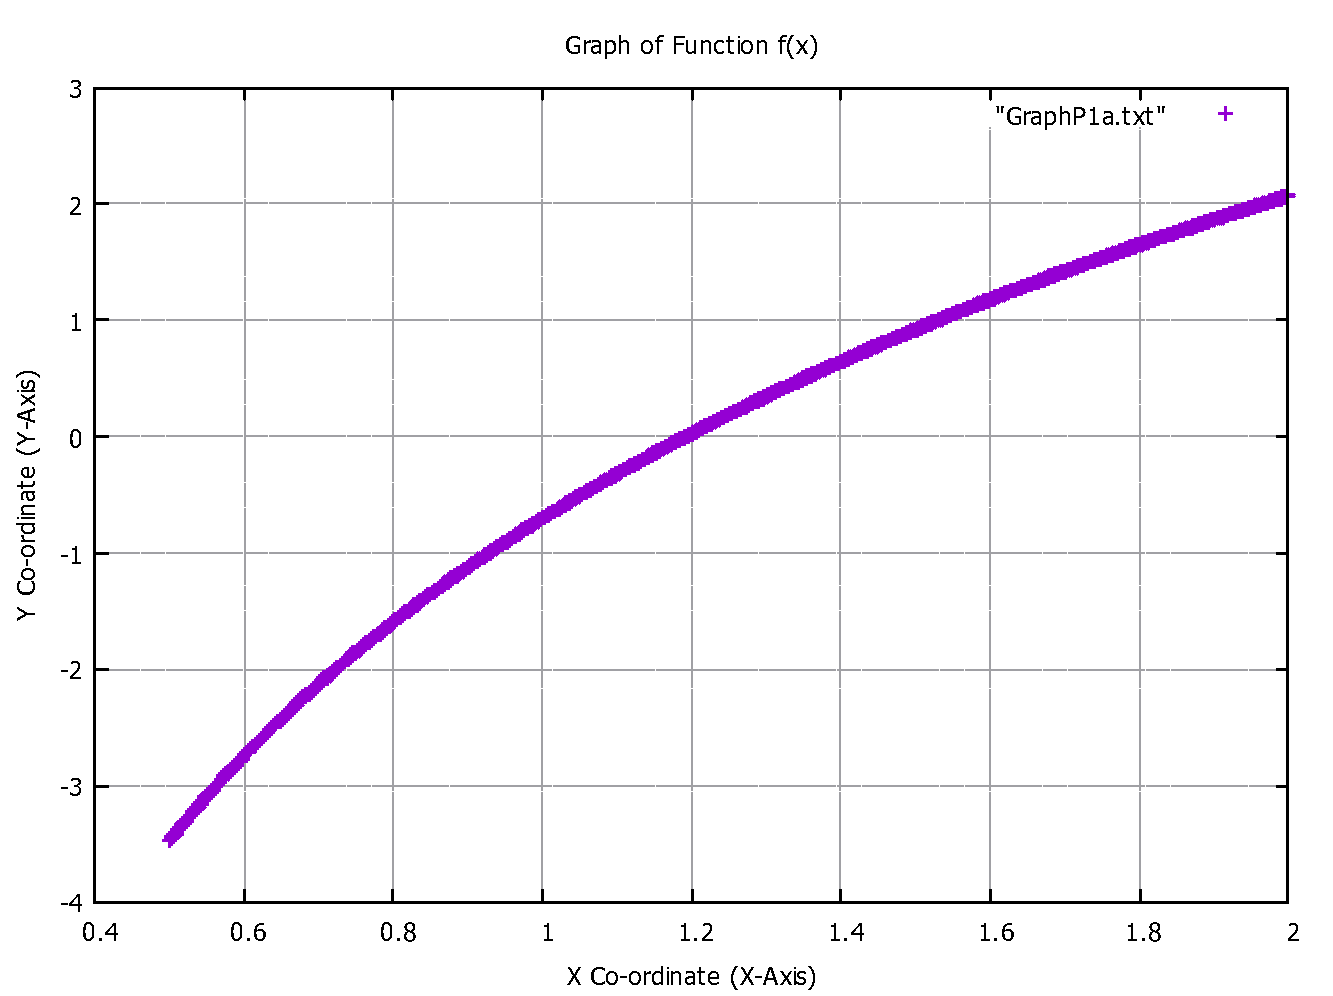
\includegraphics[width=\linewidth]{GraphP1a.pdf}
  \caption{Graph of f(x) plotted using Bisection Method CODE}
  \label{fig:fig1a}
\end{subfigure}
\begin{subfigure}{.5\textwidth}
  \centering
  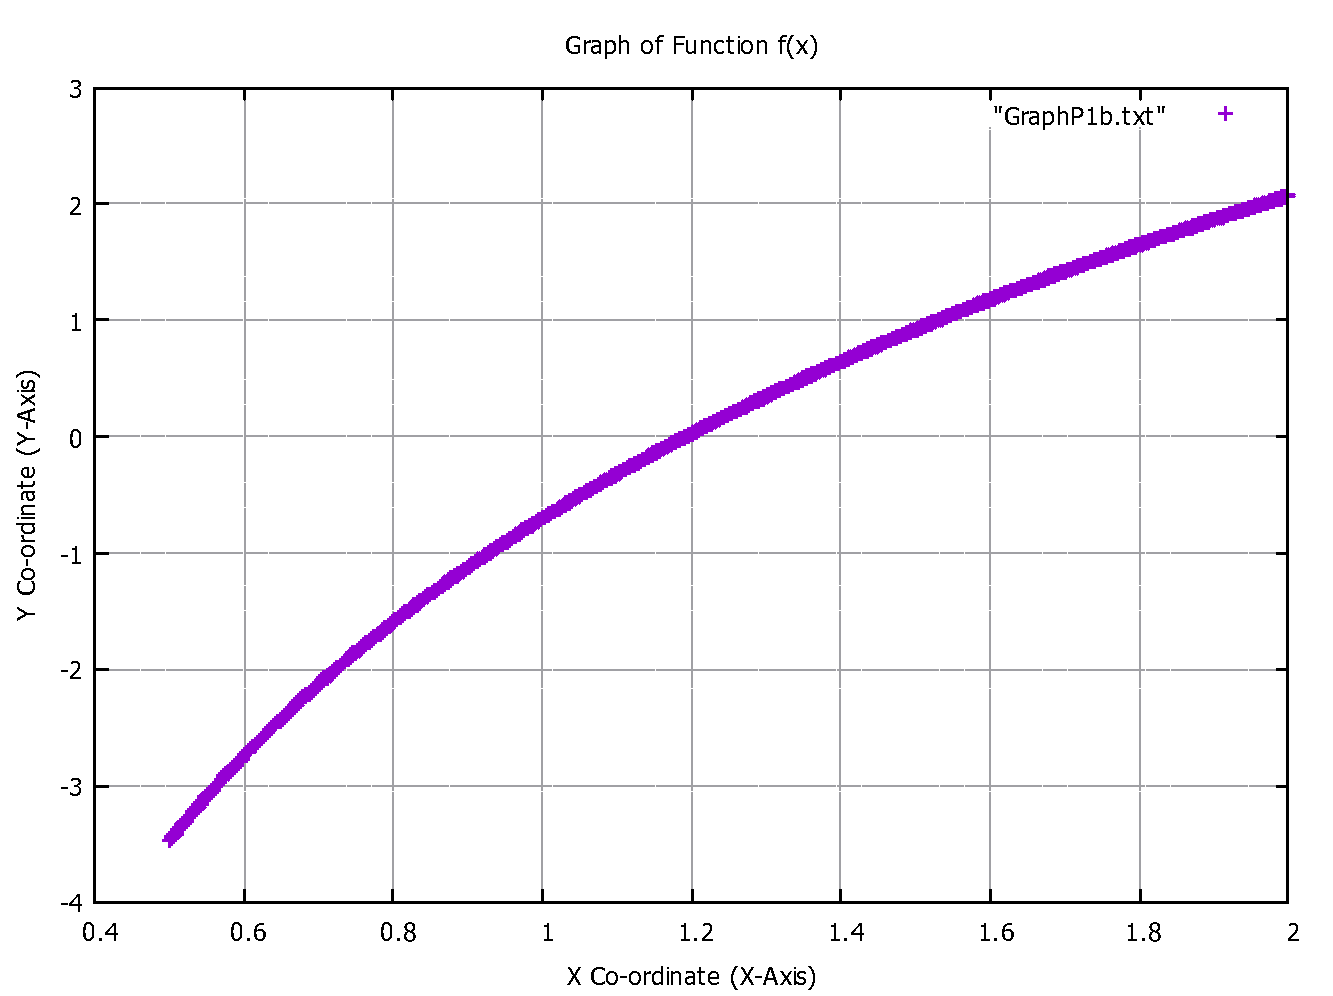
\includegraphics[width=\linewidth]{GraphP1b.pdf}
  \caption{Graph of f(x) plotted using False Position CODE}
  \label{fig:fig1b}
\end{subfigure}
\caption{Graph of f(x) }
\label{fig:Graph1}
\end{figure}

Now I shall plot the graphs showing the error percentage as a function of the number of iterations considered while approximating the roots of $f(x)=0$ In Figure~\ref{fig:fig2a} and~\ref{fig:fig2b}. The results are also summarized in Table~\ref{tab:tab1}.

\begin{figure}[ht]
\begin{subfigure}{.5\textwidth}
  \centering
  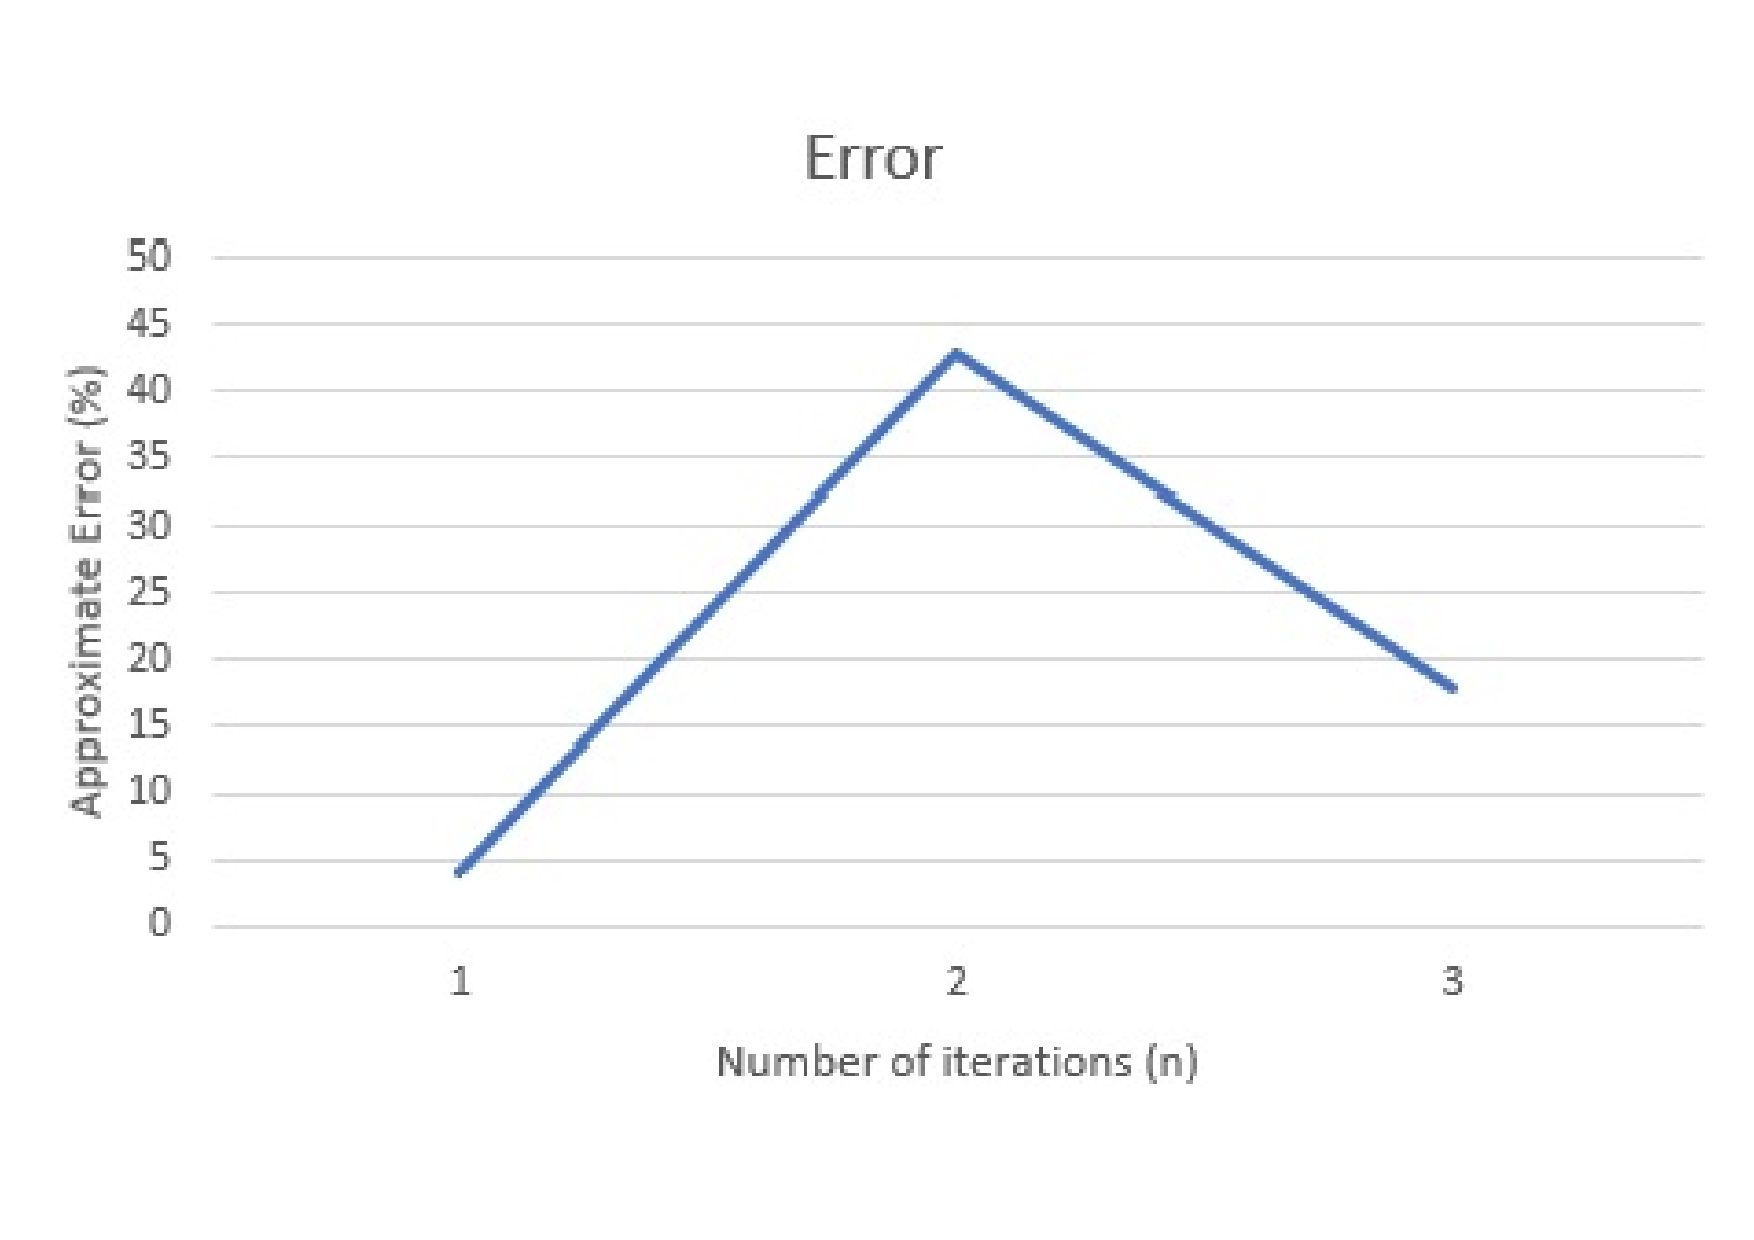
\includegraphics[width=\linewidth]{ApproxError1a.pdf}
  \caption{Approximate Error vs No. of iterations for Bisection Method}
  \label{fig:fig2a}
\end{subfigure}
\begin{subfigure}{.5\textwidth}
  \centering
  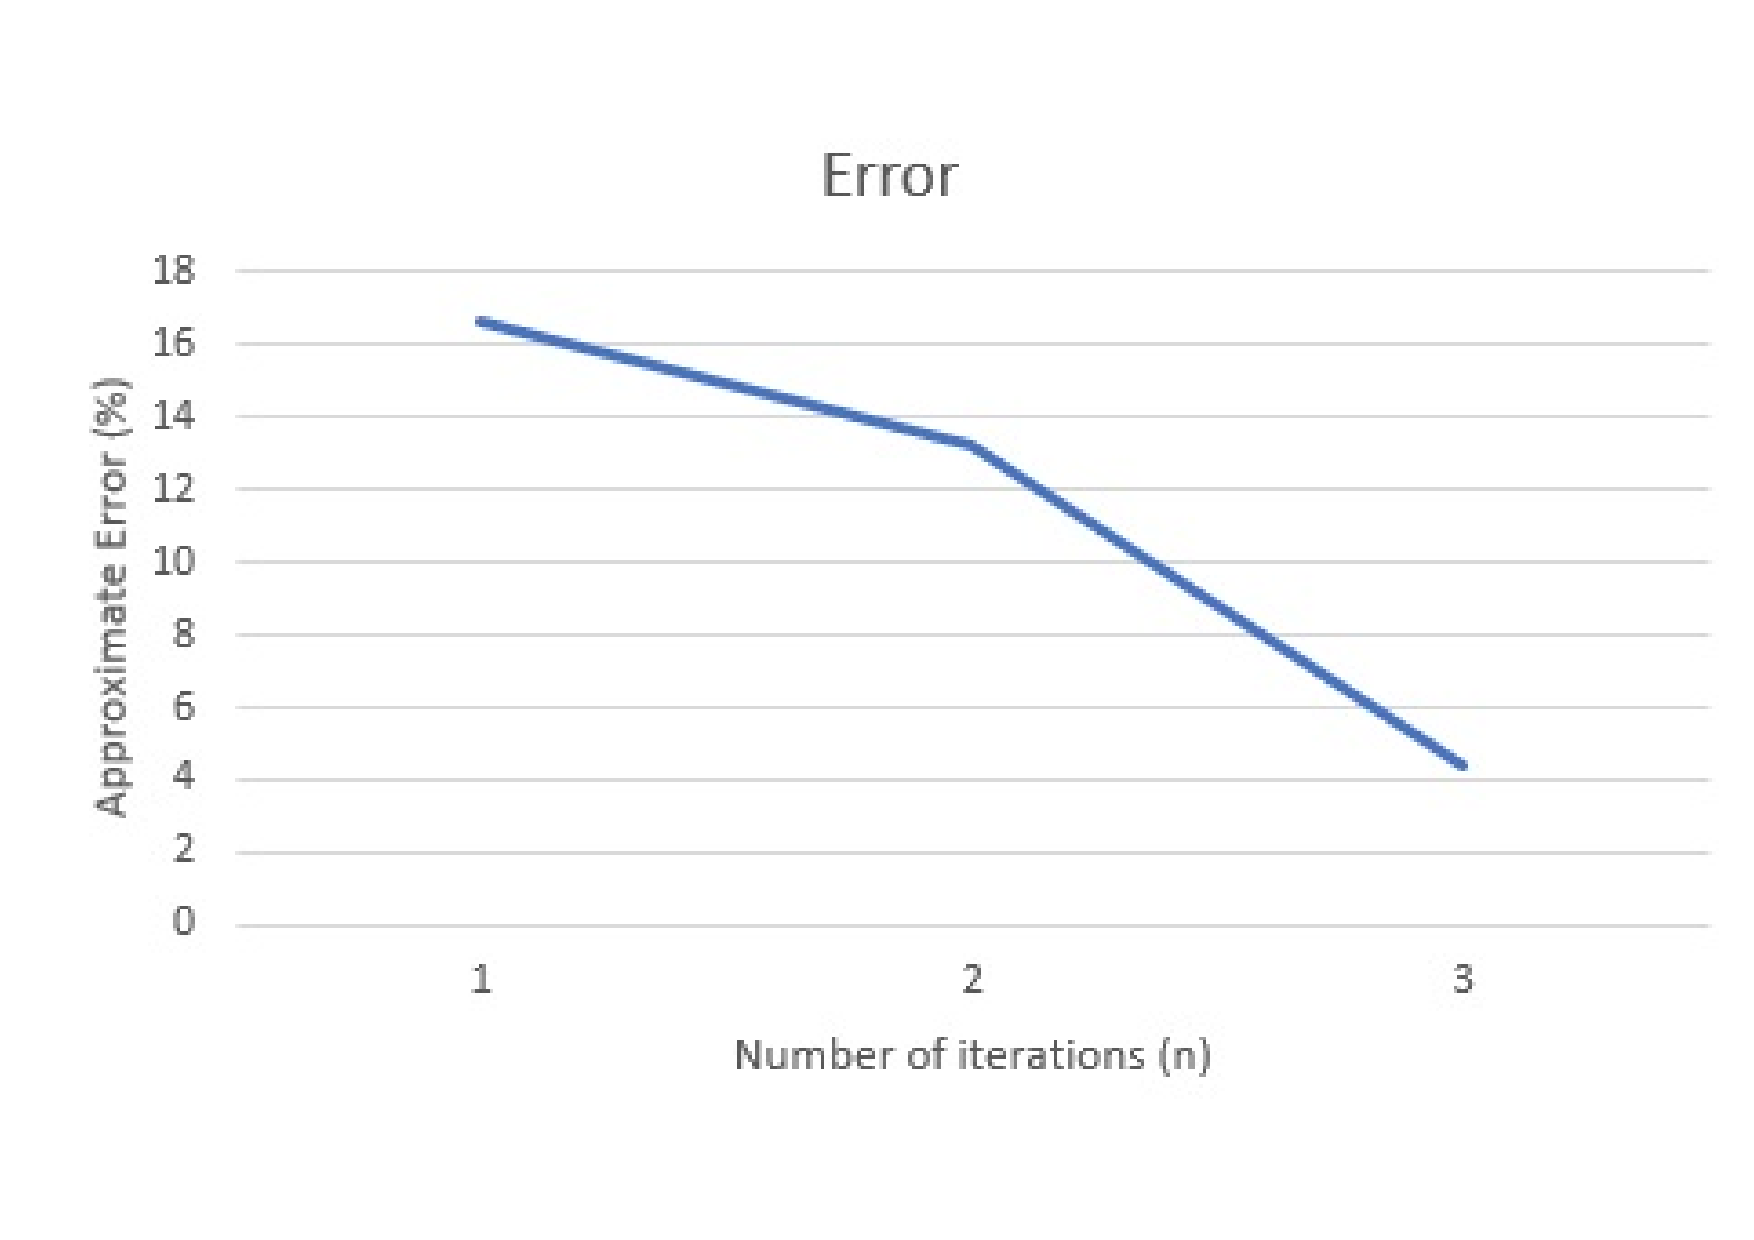
\includegraphics[width=\linewidth]{ApproxError1b.pdf}
  \caption{Approximate Error vs No. of iterations for False Position Method}
  \label{fig:fig2b}
\end{subfigure}
\caption{Approximate Error (in percent) vs Number of iterations considered while approximating the roots of $f(x)=0$.}
\label{fig:q1}
\end{figure}

\begin{figure}[ht]
\begin{subfigure}{.5\textwidth}
  \centering
  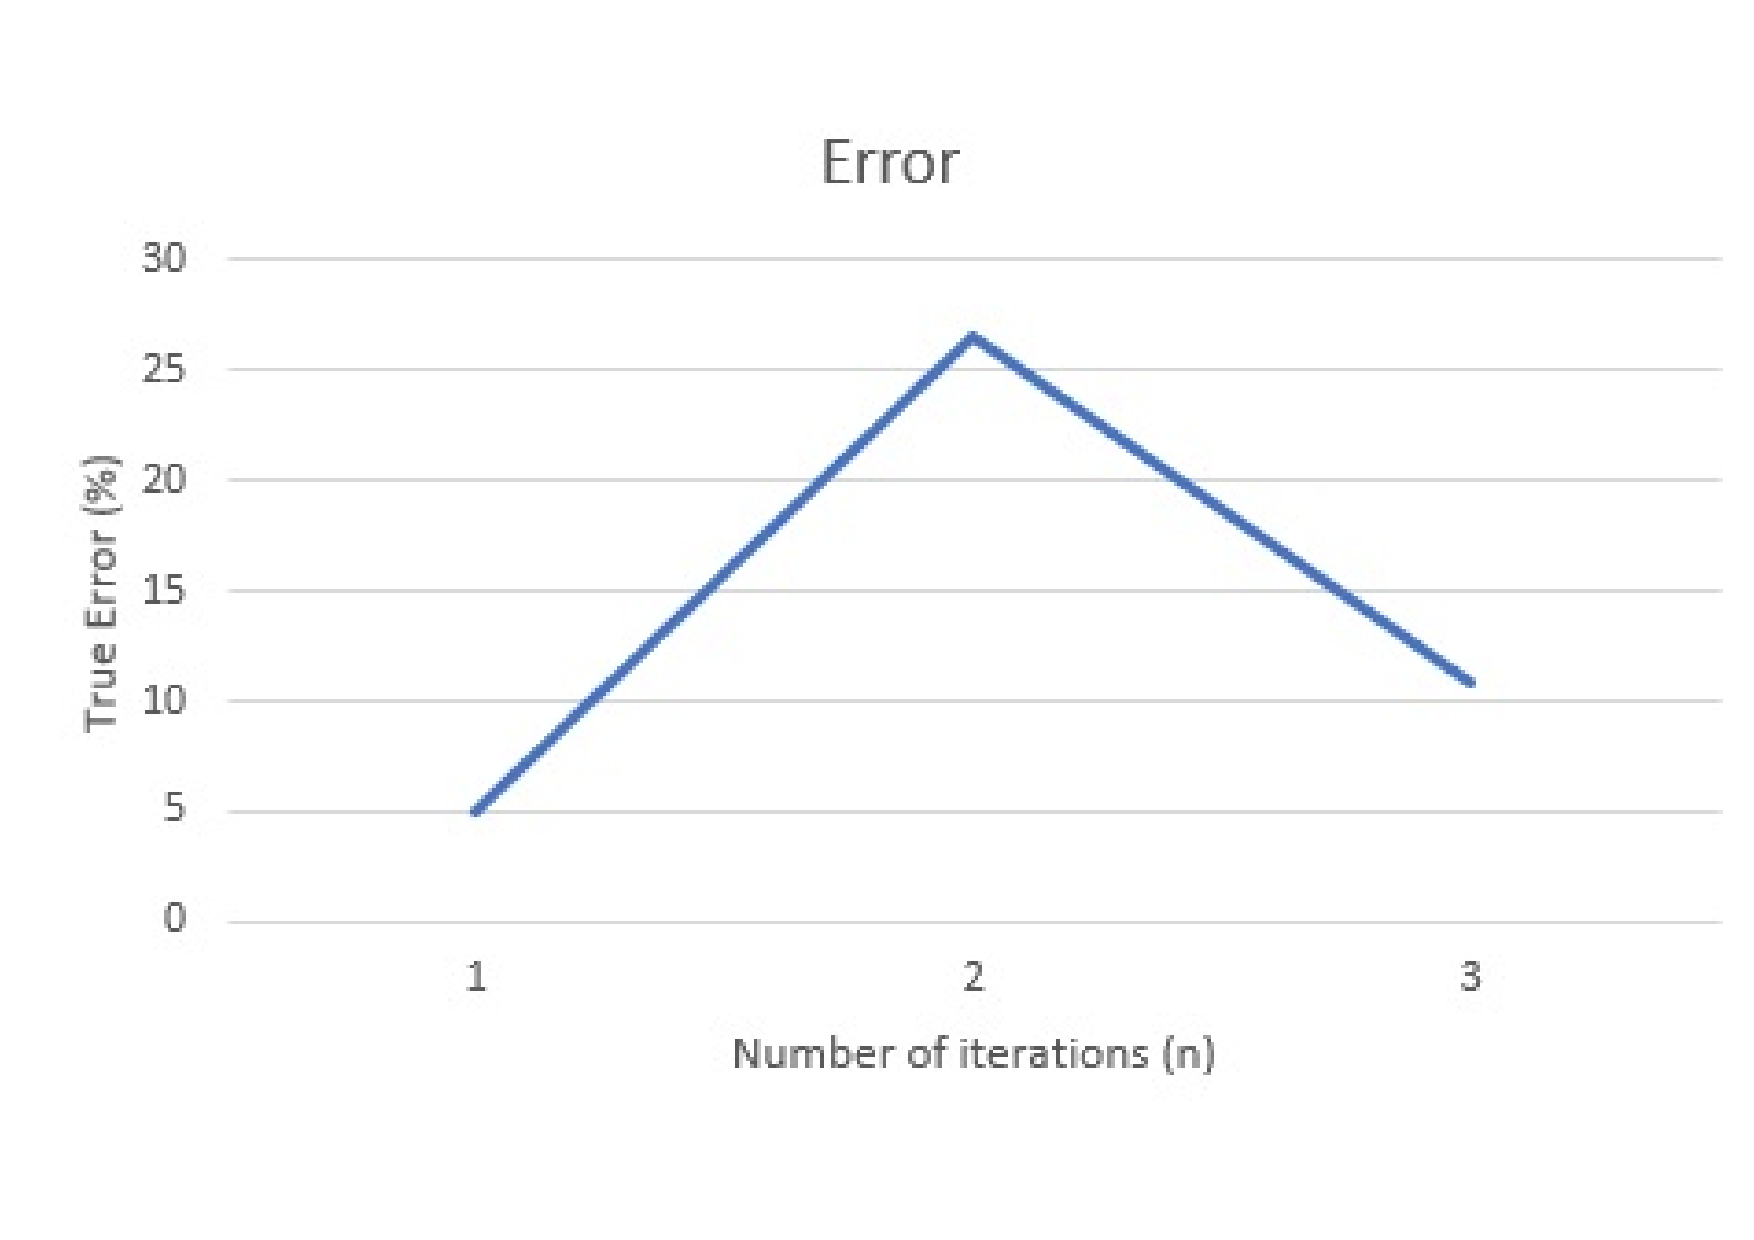
\includegraphics[width=\linewidth]{TrueError1a.pdf}
  \caption{True Error vs No. of iterations for Bisection Method}
  \label{fig:fig82a}
\end{subfigure}
\begin{subfigure}{.5\textwidth}
  \centering
  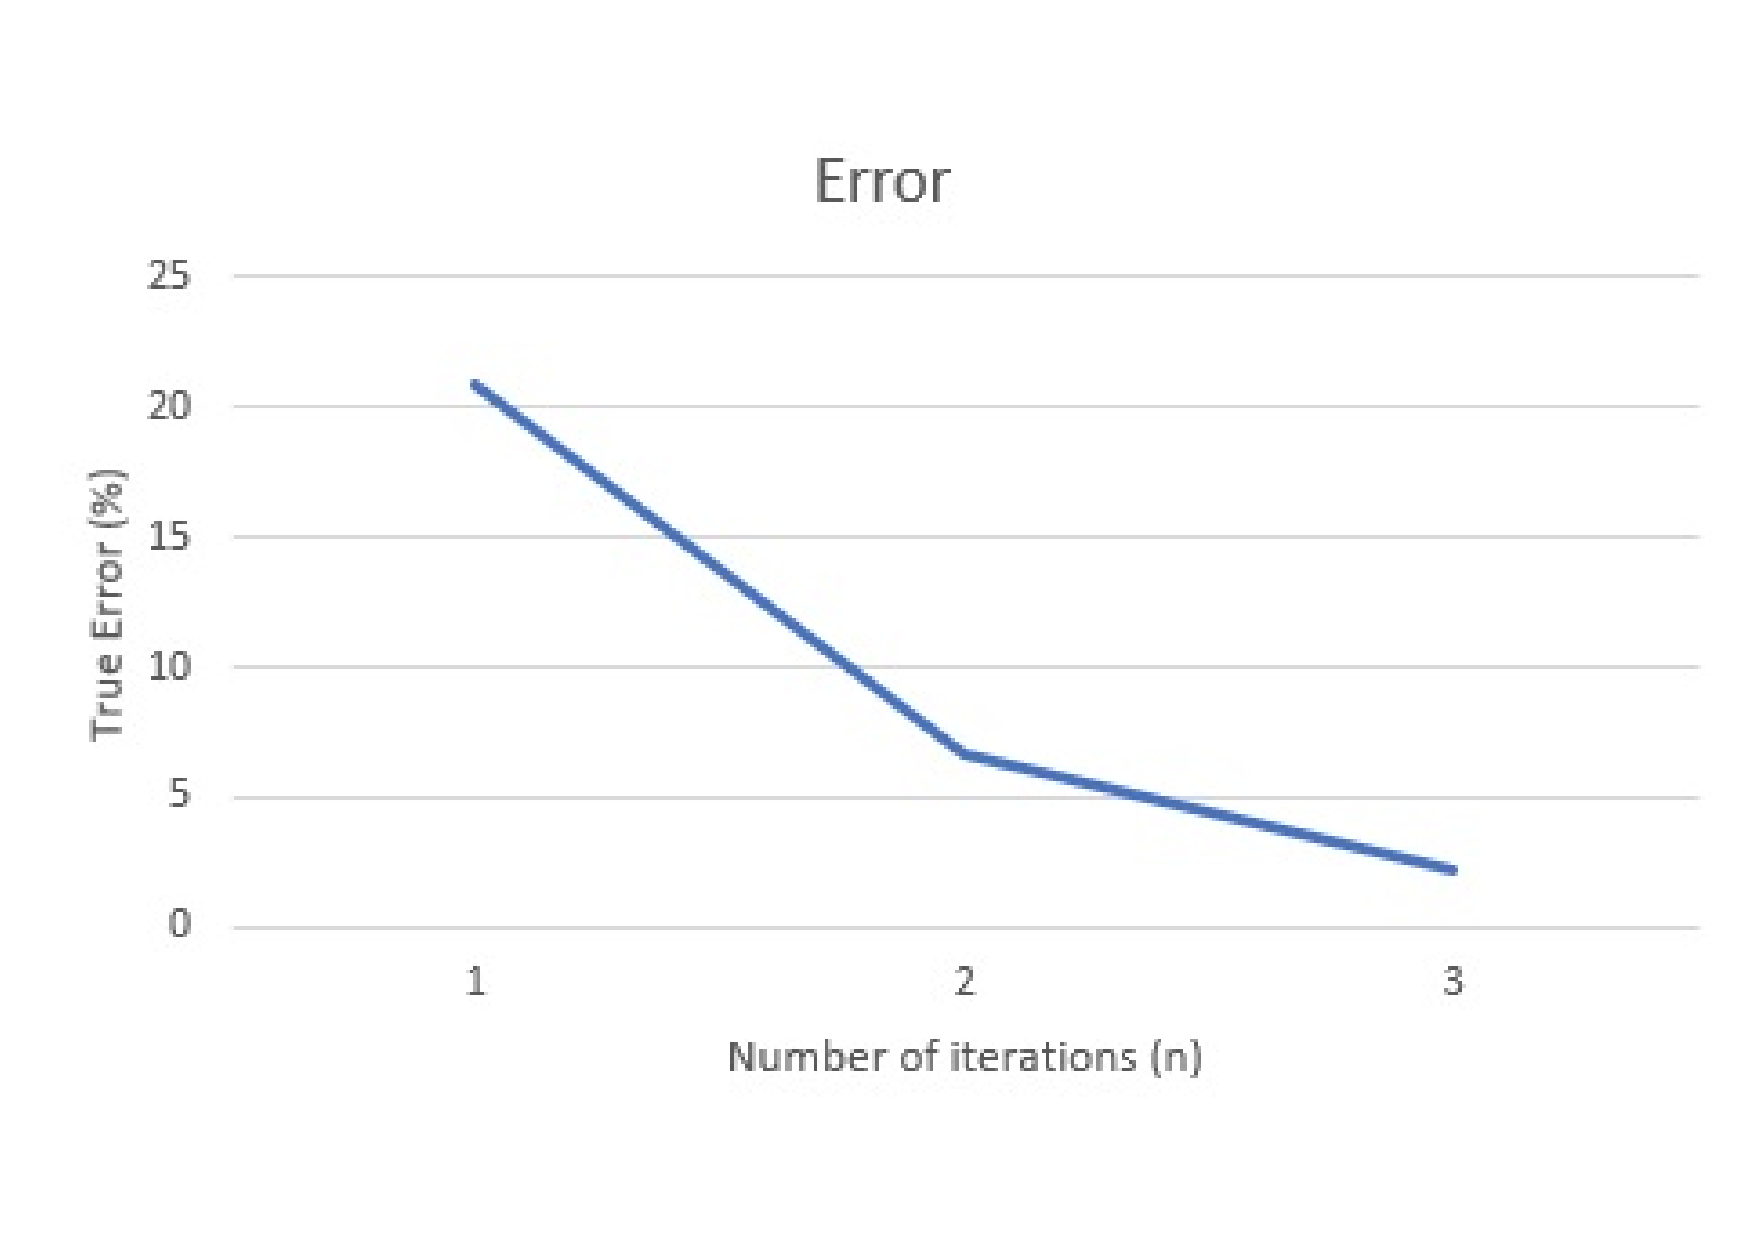
\includegraphics[width=\linewidth]{TrueError1b.pdf}
  \caption{True Error vs No. of iterations for False Position Method}
  \label{fig:fig82b}
\end{subfigure}
\caption{True Error (in percent) vs Number of iterations considered while approximating the roots of $f(x)=0$.}
\label{fig:q81}
\end{figure}


\begin{table}[!htb]
    \caption{Approximate Error percentage vs number of iterations ($n$)}
    \centering
    \begin{tabular}{ccc}
    \toprule
    \textbf{$n$}& \textbf{Error in Bisection Method }& \textbf{Error in False Position Method }   \\
    \midrule
         1 & 4.000000 &  16.629250\\
         2 & 42.857143 & 13.221583\\
         3 & 17.647059 & 4.413659 \\
    \bottomrule
    \end{tabular}
    \label{tab:tab1}
\end{table}

\begin{table}[!htb]
    \caption{True Error percentage vs number of iterations ($n$)}
    \centering
    \begin{tabular}{ccc}
    \toprule
    \textbf{$n$}& \textbf{Error in Bisection Method}& \textbf{Error in False Position Method}   \\
    \midrule
         1 & 4.932147 &  20.827581\\
         2 & 26.547497 & 6.717799\\
         3 & 10.807675 & 2.206741 \\
    \bottomrule
    \end{tabular}
    \label{tab:tab1}
\end{table}
%%%%%%%%%%%%%%%%%%%%%%%%%%%%%%%%%%%%%%%%%%%%%%%%%%%%%%

\subsection{Inferences}
I deduce the following inferences from this problem:
\begin{itemize}
    \item [1] The sharp decline in the error percentage, as a function of $n$ in Figure~\ref{fig:fig2a} and Figure~\ref{fig:fig2b} shows that the approximate error decreases as the number of iterations increases. The same conclusion can be drawn from the true error graph, the error decreases as the number of iterations increase as evident from Figure~\ref{fig:fig82a} and Figure~\ref{fig:fig82b}. The first iteration throws an error by comparing with the root we are expecting after the iterative procedure is complete. 
    \item [2] However, we see that the False Position Method gives a better efficiency compared to the Bisection Method for a given iteration. This is generally true for monotonic curves having a single root.
    \item [3] The Bisection Method is a slow converging root finding method. The False Position is a faster method yet not the fastest. 
    \item [4] We also deduce that the False Position Method converges faster than the Bisection Method. 
\end{itemize}

%%%%%%%%%%%%%%%%%%%%%%%%%%%%%%%%%%%%%%%%%%%%%%%%%%%%%%

\subsection{Code}
The code used for the problem is mentioned in Listing~\ref{listing:1} and  Listing~\ref{listing:2}

\begin {itemize}
\item [(1)] Bisection Method CODE
\end {itemize}
\inputminted[breaklines,
 mathescape,
 linenos,
 numbersep=5pt,
 frame=single,
 numbersep=5pt,
 xleftmargin=0pt]{c}{Bisection1.c}
 \captionof{listing}{Code snippet used in the problem.}
\label{listing:1}

\begin {itemize}
\item [(2)] False Position Method CODE
\end {itemize}
\inputminted[breaklines,
 mathescape,
 linenos,
 numbersep=5pt,
 frame=single,
 numbersep=5pt,
 xleftmargin=0pt]{c}{FalsePosition1.c}
 \captionof{listing}{Code snippet used in the problem.}
\label{listing:2}

%%%%%%%%%%%%%%%%%%%%%%%%%%%%%%%%%%%%%%%%%%%%%%%%%%%%%%

\subsection{Contributions}
In the above problem, \textit{my original contributions} are - 
\begin{itemize}
    \item Designing of the Algorithm and Code
    \item Plotting of the graph on GNU Plot and MS Excel
    \item Analysis of True Error and Approximate Error
    \item Tabulation of Results and Errors
    \item Drawing conclusions by looking at the Result obtained and Error Analysis.
\end{itemize}

\subsection{Alternate Methods}
\begin{itemize}
\item [1] We need to tackle the situation of multiple roots and tangential roots, which cannot be easily detected by the Bisection Algorithm or the False Position Algorithm in its present form and needs suitable modifications. This can be considered as one of the pitfalls of the Bracketing Method in the case of evaluation of multiple roots in a Bracketed interval or a tangential root. 
\item [2] The Bisection Algorithm is a slowly converging root finding technique. Thus, its time complexity is higher as evident from the True Error v/s Number of iterations graph in Figure~\ref{fig:fig82a}. This is not suitable for cases in which the result is required immediately. 
\end{itemize}
%%%%%%%%%%%%% END OF QUESTION 1 %%%%%%%%%%%%%%%%%%%%
\newpage
\section{Problem 2}
Sketch the following function in a sensible range to understand its nature and then employ the Newton-Raphson method to determine a real root for
\begin{align}
    f(x) = -2 + 6x - 4x^2 + 0.5x^3
\end{align} 
using initial guesses of
\begin{itemize}
    \item [(a)] 4.2 and
    \item [(b)] 4.43.
\end{itemize}
Run the algorithm for 50 iterations in each case and plot the approximate error percentages as a function of iteration number. Comment on your results and discuss any peculiarities you observe in your results. 

\subsection{Approach}

We solve the given problem using the Newton-Raphson method as stated in the question. 

In this problem, we find the roots of $f(x)=0$ 

%%%%%%%%%%%%%%%%%%%%%%%%%%%%%%%%%%%%%%%%%%%%%%%%%%%%%%

\subsection{Algorithm}
In this section, I present the pseudocode/flowchart of the algorithm used to solve the problem.

The pseudocode for finding the roots of f(x)=0 is provided in Algorithm~\ref{alg3}.
\begin{center}
\begin{algorithm}[H]\label{alg3}

\SetAlgoLined

Input $x_1,f,f'$ \\
$x_{rold} \gets x_1$ \\
$ITER_{MAX}$ \gets 50 \\
count = 1 \\
\While {count <=$ITER_{MAX}$} {
$x_{rnew} \gets x_{rold} - \frac{f(x_{rold})}{f'(x_{rold})}$ \;
\If{$x_{rnew}$ \neq 0}{
$e_a \gets \frac{|x_r-x_{rold}|}{|x_r|} * 100$ \;
}
$x_{rold} \gets x_{rnew}$\;
count++ \;
return ${x_{rnew}}$\;
}

 \caption{Approximating roots of $f(x)=0$ using Newton-Raphson Method}
\end{algorithm} 
\end{center}

%%%%%%%%%%%%%%%%%%%%%%%%%%%%%%%%%%%%%%%%%%%%%%%%%%%%%%
\subsection{Results}

We find out that the root of $f(x)=0$ is $x=0.474572$ with Errors as mentioned in Table~\ref{tab:tab2}.

In this section, I plot the graph of the function f(x) in the range [-5,5] using GNU plot in Figure~\ref{fig:3}
\begin{figure}
  \centering
    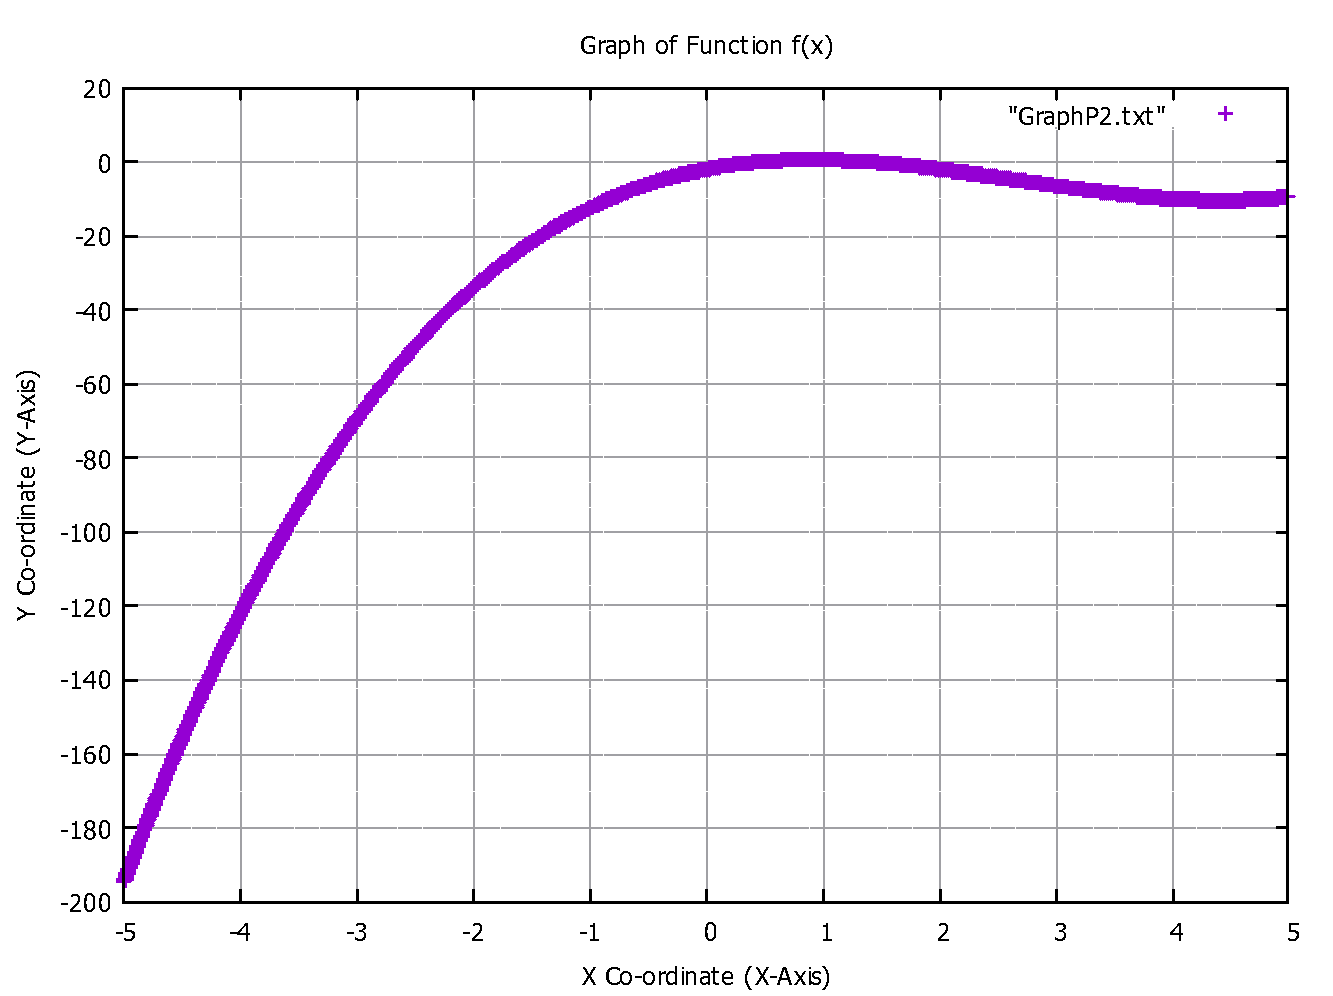
\includegraphics[width=\linewidth]{GraphP2.pdf}
    \caption{Graph of f(x)}
    \label{fig:3}
\end{figure}

Now I shall plot the graphs showing the error percentage as a function of the number of iterations considered while approximating the roots of $f(x)=0$ In Figure~\ref{fig:fig4a} and~\ref{fig:fig4b}. The results are also summarized in Table~\ref{tab:tab2}.

\begin{figure}[ht]
\begin{subfigure}{.5\textwidth}
  \centering
  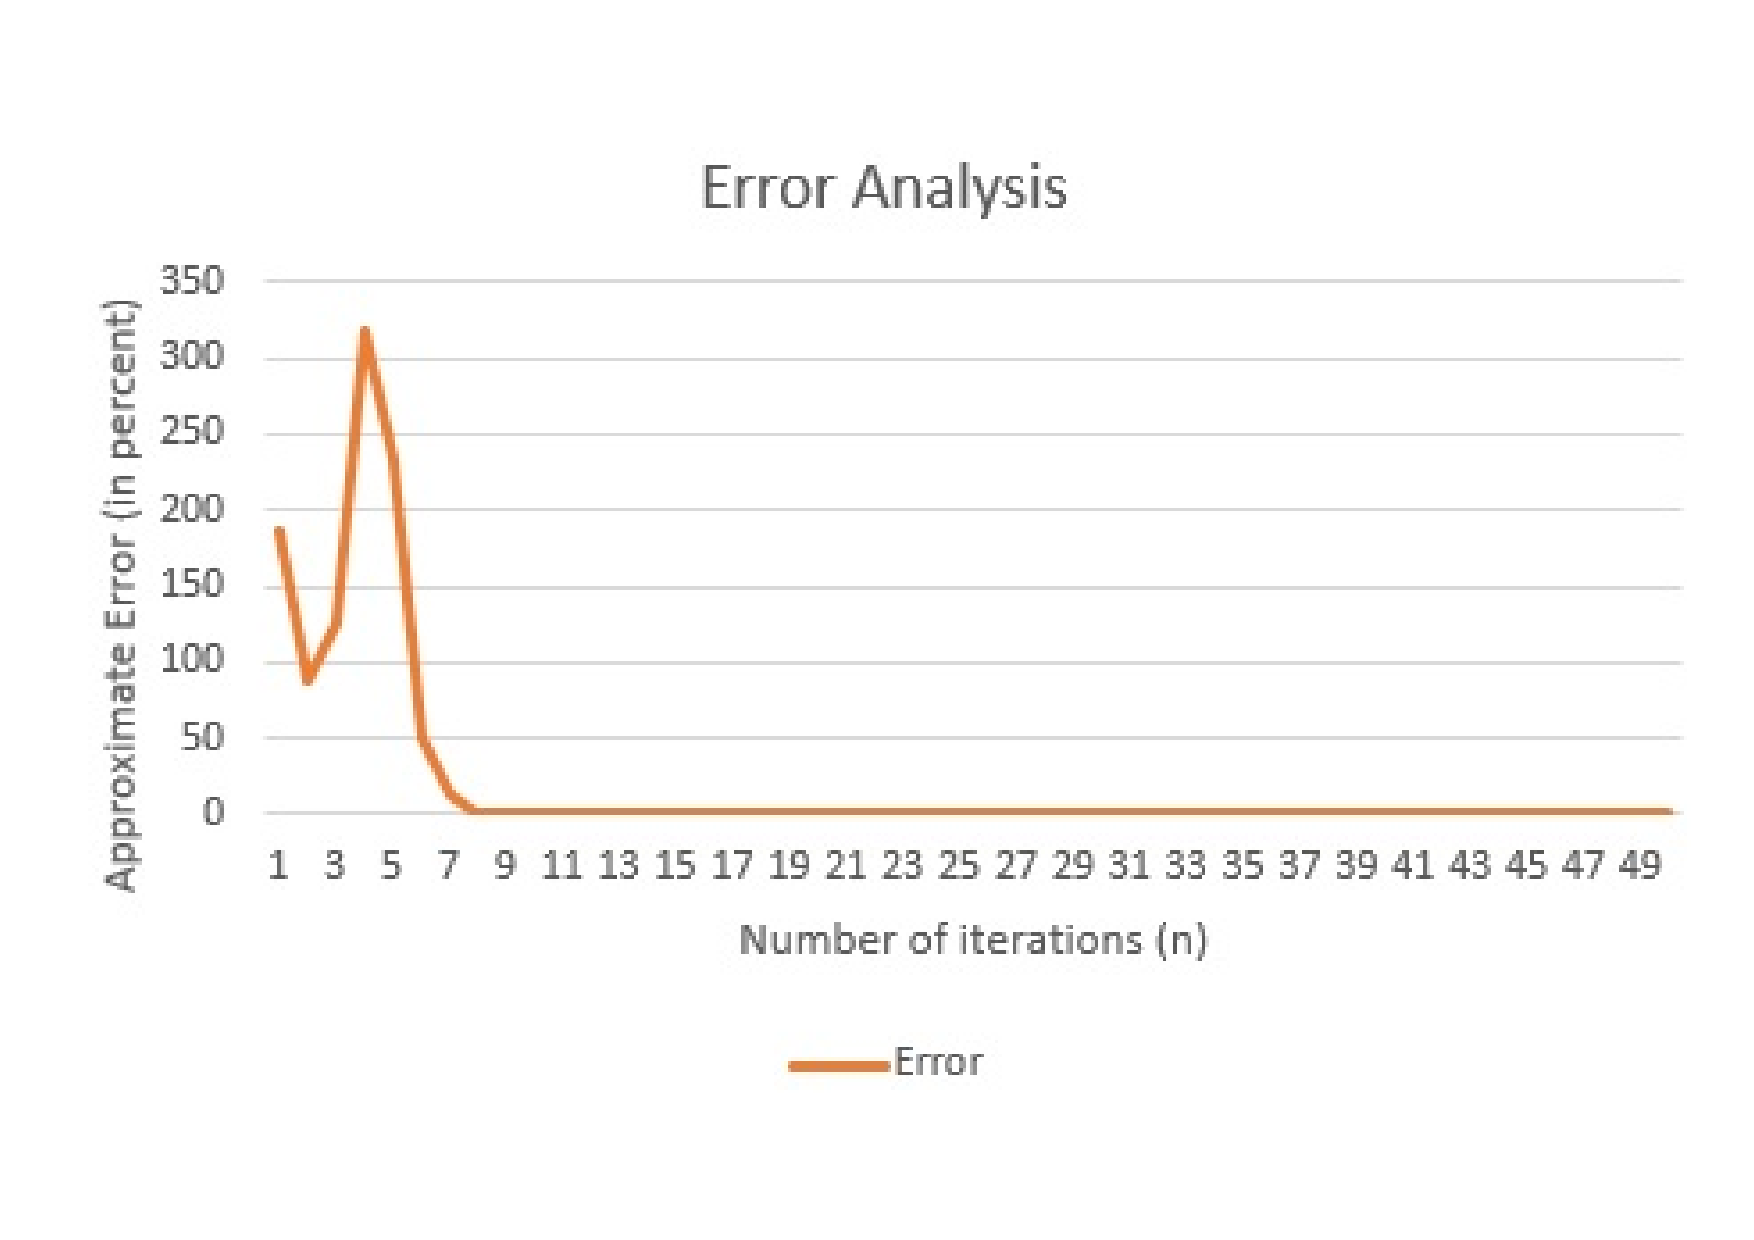
\includegraphics[width=\linewidth]{ErrorP2a.pdf}
  \caption{Error vs No. of iterations for Newton-Rapshon Method for (a)4.2}
  \label{fig:fig4a}
\end{subfigure}
\begin{subfigure}{.5\textwidth}
  \centering
  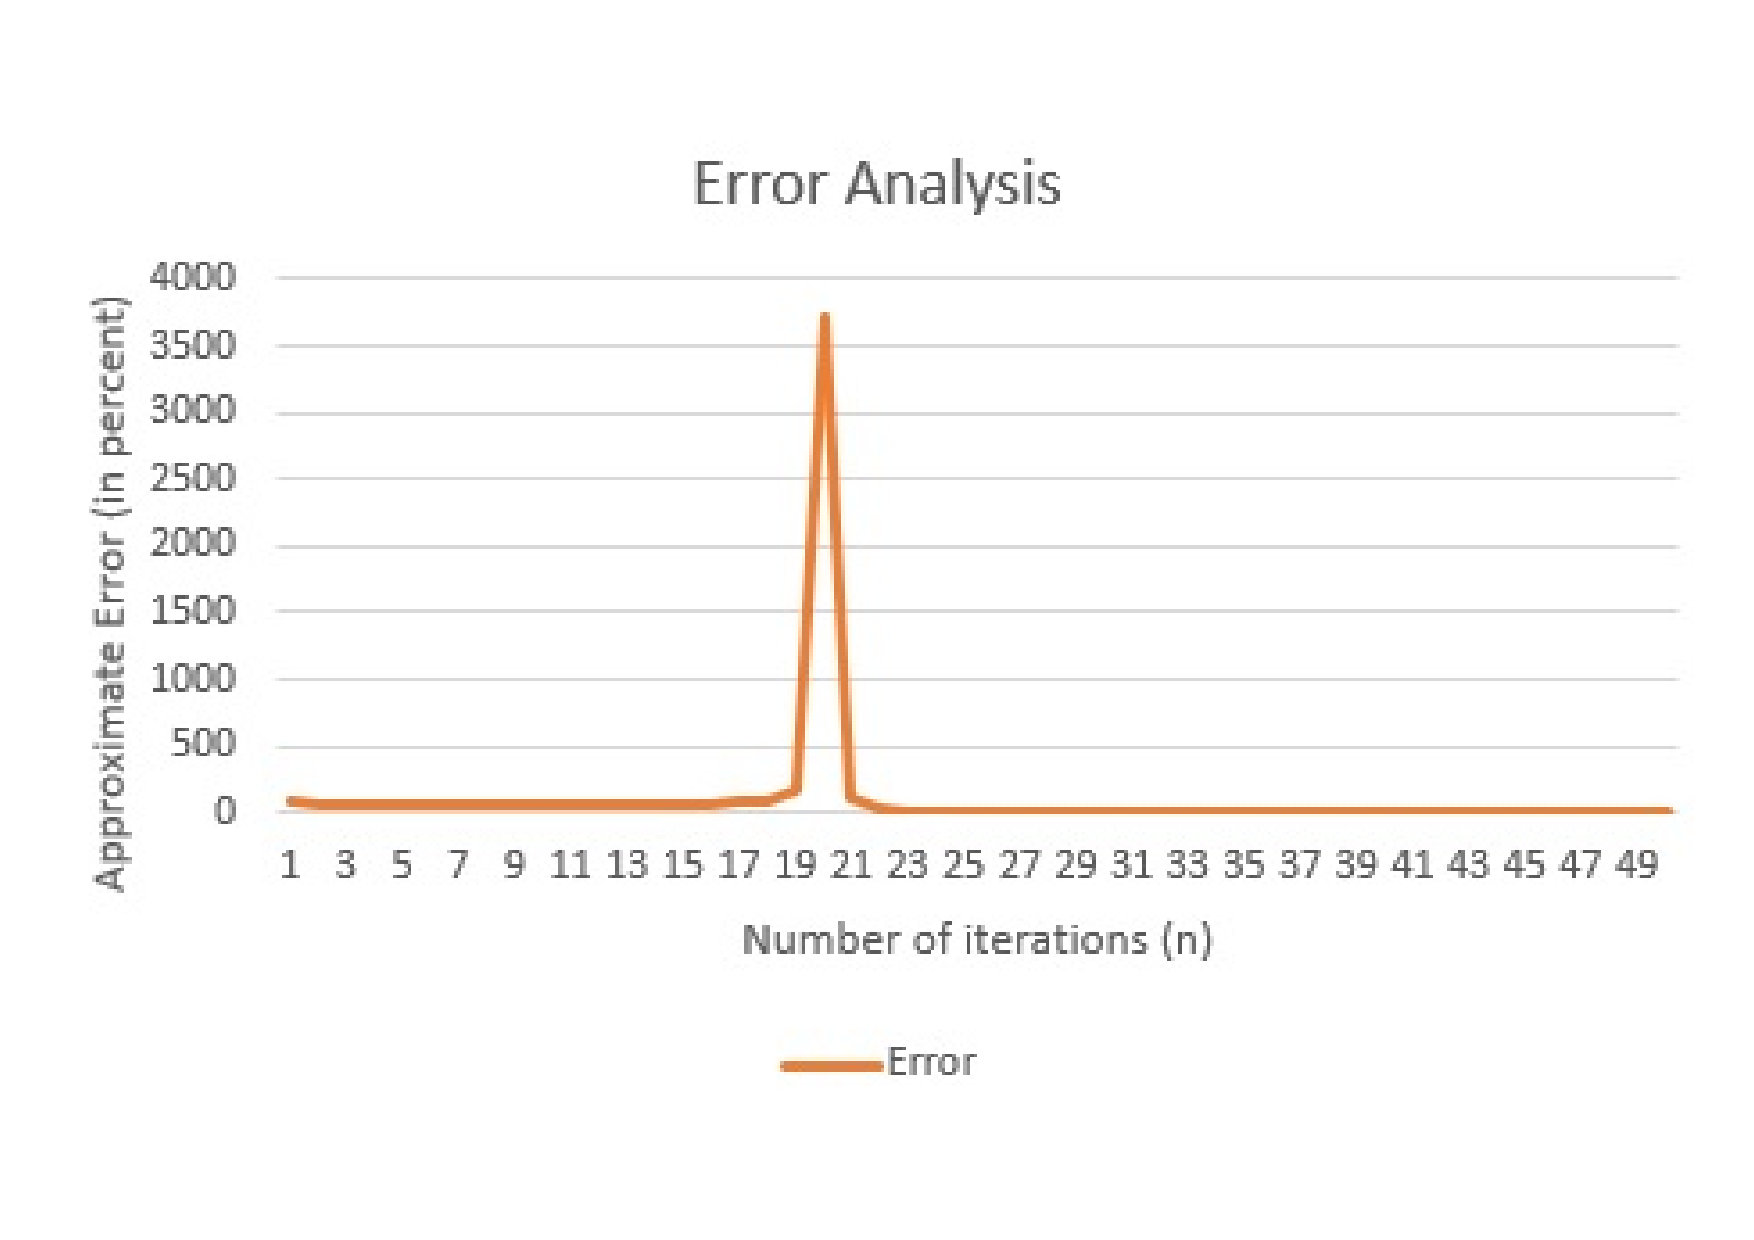
\includegraphics[width=\linewidth]{ErrorP2b.pdf}
  \caption{Error vs No. of iterations for Newton-Rapshon Method for (b)4.43}
  \label{fig:fig4b}
\end{subfigure}
\caption{Approximate Error (in percent) vs Number of iterations considered while approximating the roots of $f(x)=0$.}
\label{fig:q2}
\end{figure}
\begin{figure}[ht]
\begin{subfigure}{.5\textwidth}
  \centering
  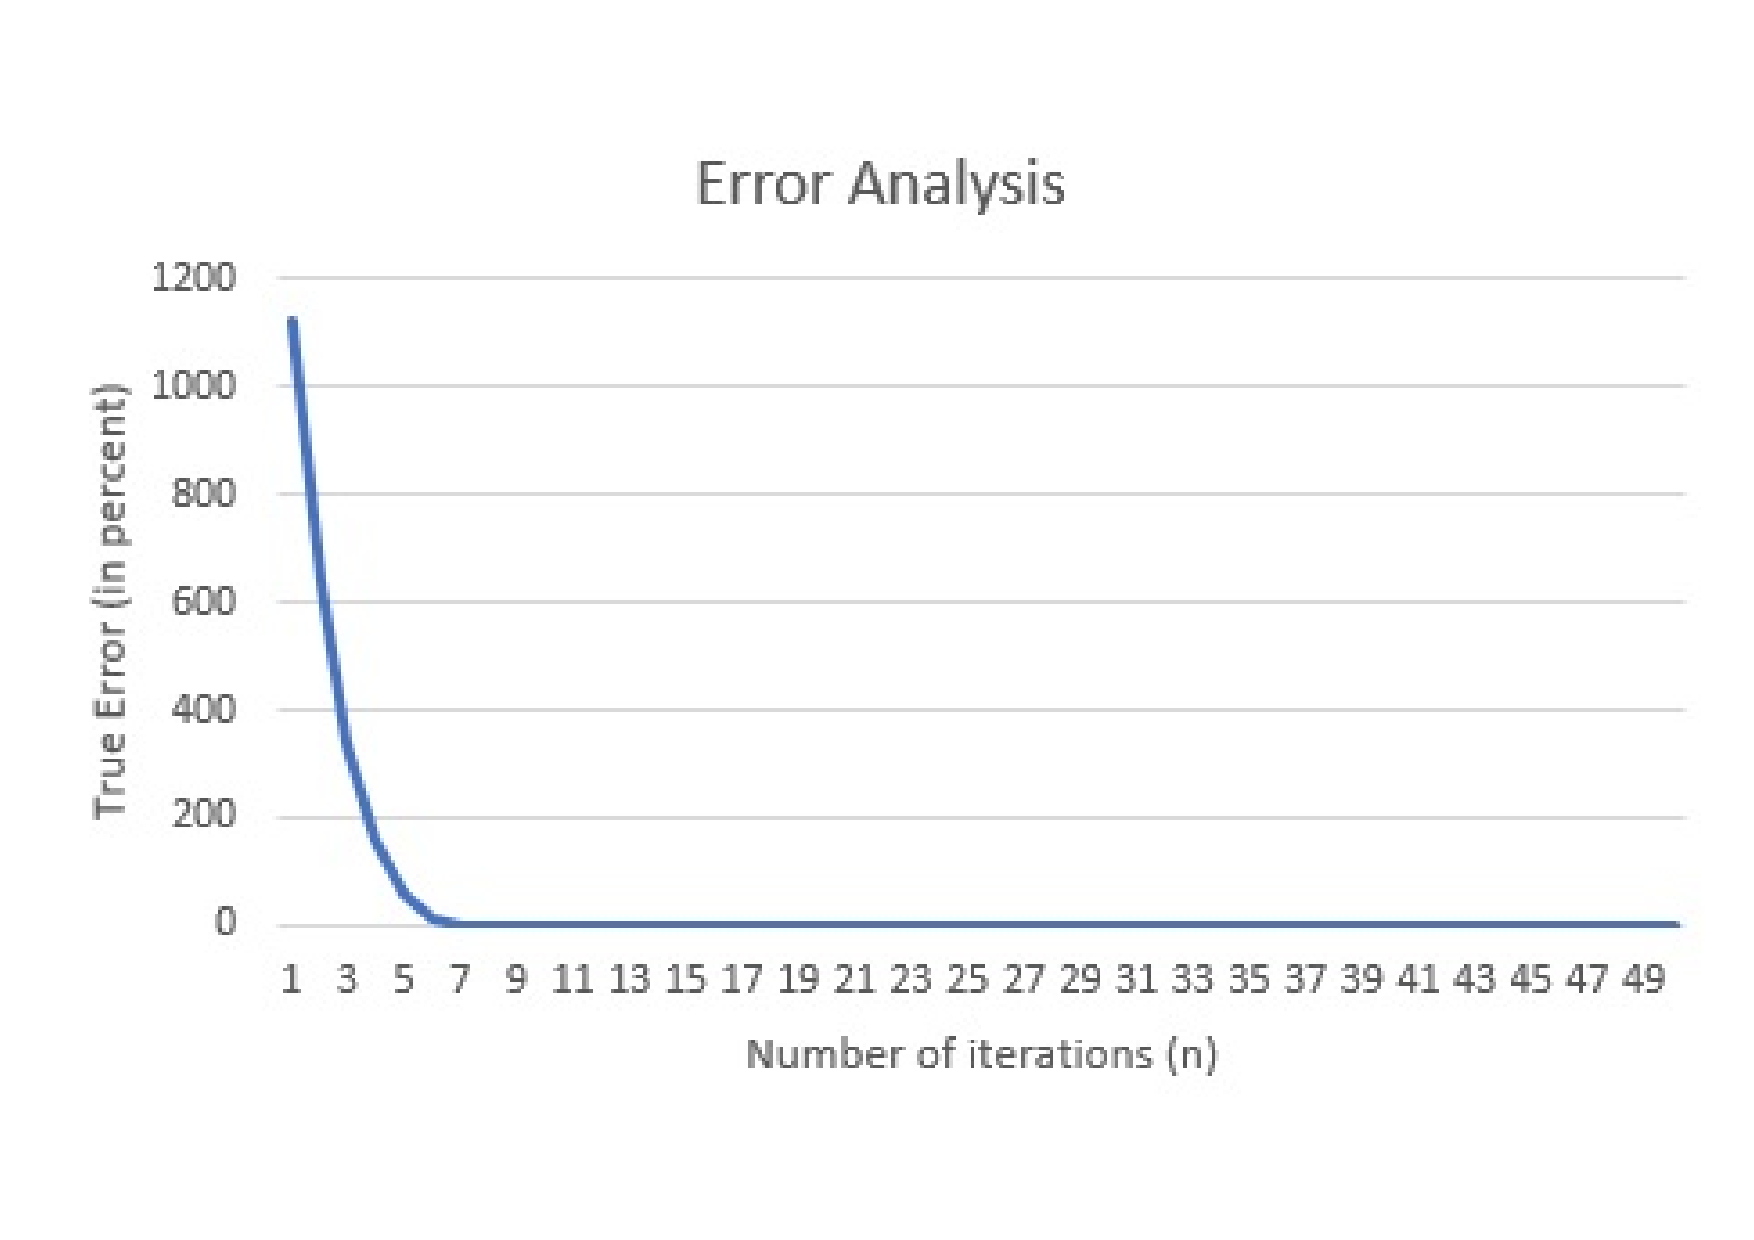
\includegraphics[width=\linewidth]{TE2a.pdf}
  \caption{True Error vs No. of iterations for Newton-Rapshon Method for (a)4.2}
  \label{fig:fig84a}
\end{subfigure}
\begin{subfigure}{.5\textwidth}
  \centering
  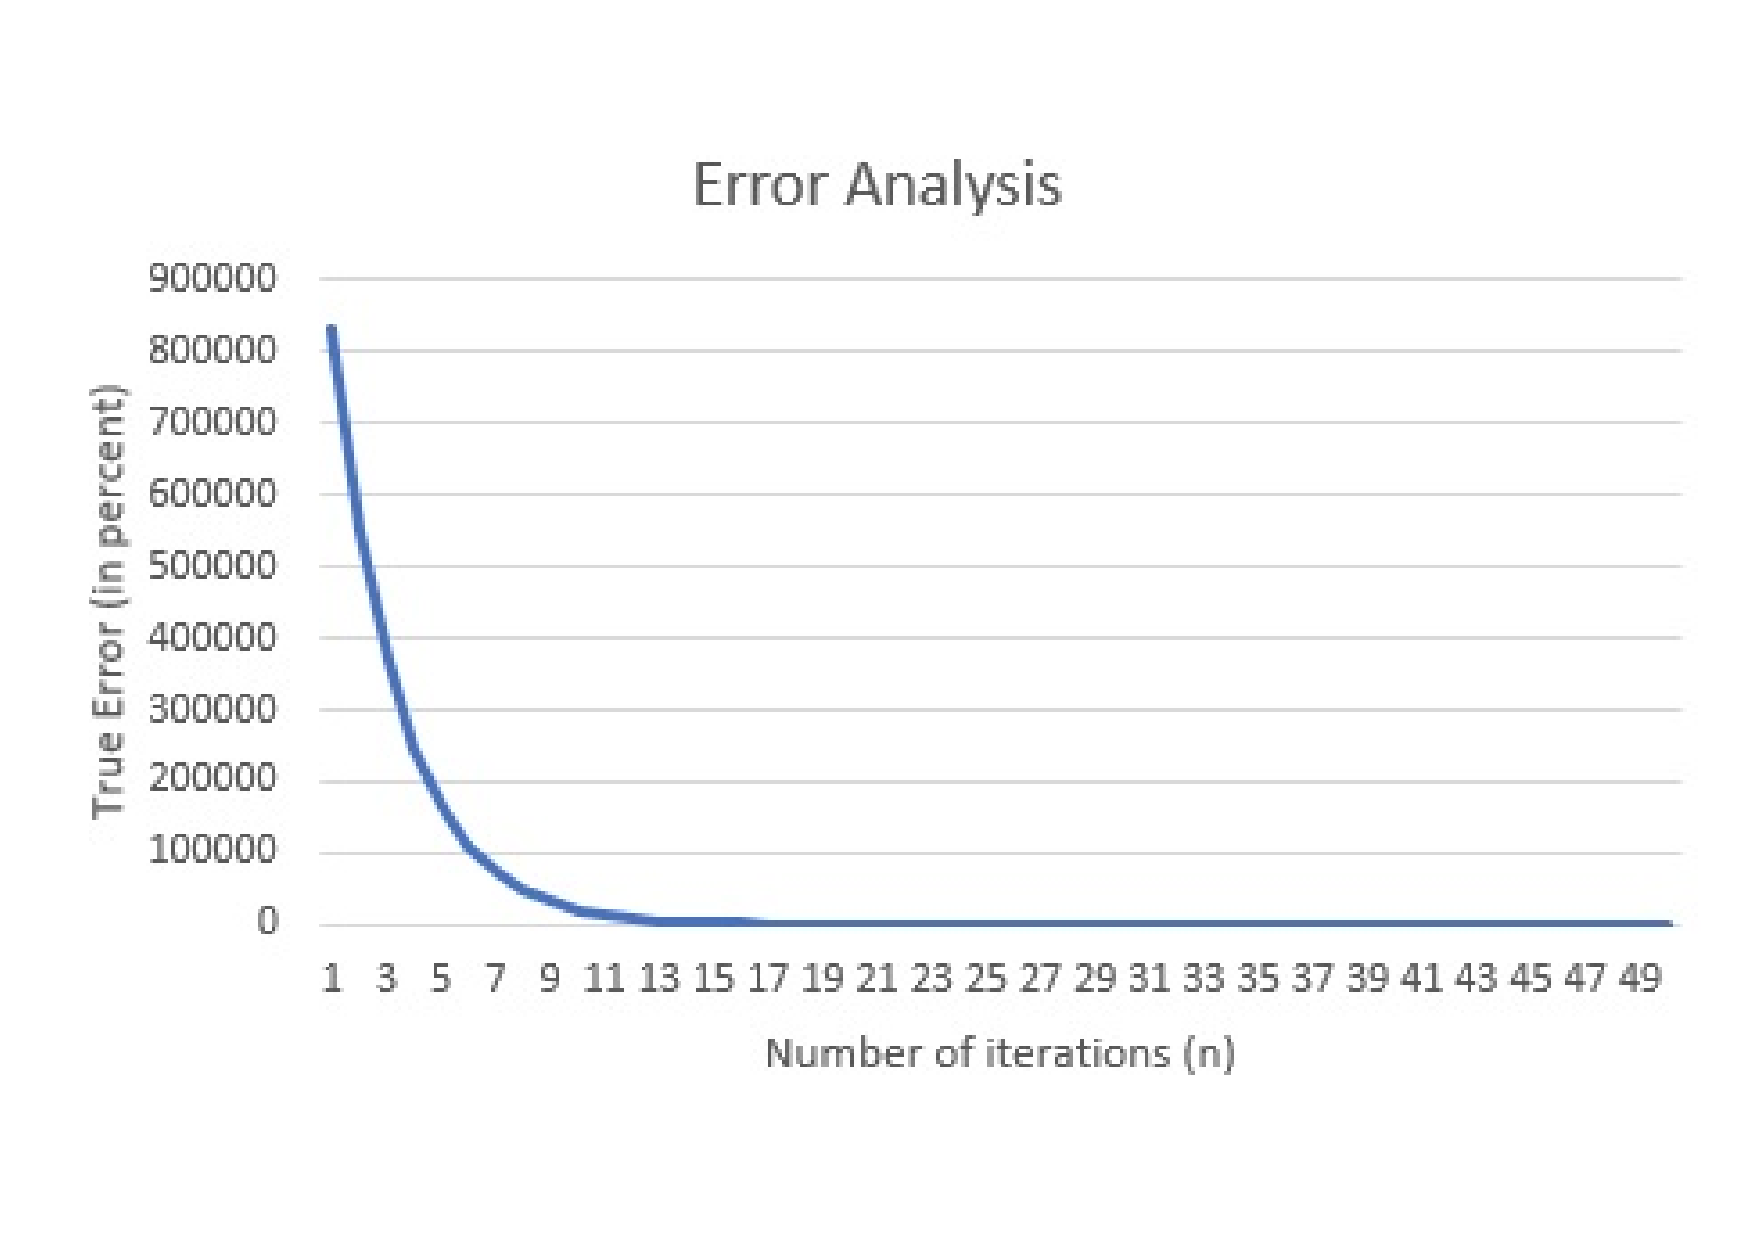
\includegraphics[width=\linewidth]{TE2b.pdf}
  \caption{True Error vs No. of iterations for Newton-Rapshon Method for (b)4.43}
  \label{fig:fig84b}
\end{subfigure}
\caption{True Error (in percent) vs Number of iterations considered while approximating the roots of $f(x)=0$.}
\label{fig:q82}
\end{figure}
\begin{table}[!htb]
    \caption{Approximate Error percentage vs Number of iterations}
    \centering
    \begin{tabular}{ccc}
    \toprule
    \textbf{$n$}& \textbf{Error Percentage (a)}& \textbf{Error Percentage (b)}   \\
    \midrule
         1 & 186.613603 & 100.112461 \\
         5 & 234.466585 & 50.171486 \\
         10 & 0.000000 & 51.314725\\
         20 & 0.000000 & 3712.744178 \\
         30 & 0.000000 & 0.000000 \\
         40 & 0.000000 & 0.000000\\
         50 & 0.000000 & 0.000000\\
    \bottomrule
    \end{tabular}
    \label{tab:tab2}
\end{table}
\begin{table}[!htb]
    \caption{True Error percentage vs Number of iterations}
    \centering
    \begin{tabular}{ccc}
    \toprule
    \textbf{$n$}& \textbf{Error Percentage (a)}& \textbf{Error Percentage (b)}   \\
    \midrule
         1 & 1121.788645 & 830139.428575 \\
         5 & 57.260460 & 163608.136912 \\
         10 & 0.000093 & 21149.006690\\
         20 & 0.000093 & 103.803492 \\
         30 & 0.000093 & 0.000093 \\
         40 & 0.000093 & 0.000093\\
         50 & 0.000093 & 0.000093\\
    \bottomrule
    \end{tabular}
    \label{tab:tab82}
\end{table}

%%%%%%%%%%%%%%%%%%%%%%%%%%%%%%%%%%%%%%%%%%%%%%%%%%%%%%

\subsection{Inferences}
We deduce the following inferences from this problem:
\begin{itemize}
    \item [1] The sharp decline in the error percentage, as a function of $n$ in Figure~\ref{fig:fig4a} and Figure~\ref{fig:fig4b} . As we increase the number of iterations, the error percentage drops down.
    \item [2] We see that the Newton-Raphson Method is an extremely fast method for  computation of the root of a function $f(x)=0$ as compared to Bisection Method and False Position Method.
    \item [3] We also spot that the error percentages in some cases exceed 100\%, which is because the present root and the previous root are of opposite sign. The difference comes out to be more than the present root, thus, the error percentage unexpectedly goes beyond 100\%.
    \item [4] Though the graph of the function $f(x)=0$ clearly shows three distinct roots, yet the Newton Raphson Method gives us only one root for values (a) 4.2 and (b) 4.43 which is $x=0.474572$. A suitable explanation for the same would be that the tangent line intersects at a negative x intercept and this new point slowly climbs towards the nearest root which is $x=0.474572$. This explains both the error exceeding 100\% as well as only one root predicted by the Newton Raphson Algorithm which is nearest to the origin. 
    \item [5] The point (b) x= 4.43 shows a peak of error at somewhere around 20 iterations because the point (b) x=4.43 is a point near the minima of the curve, thus tangent line is nearly horizontal. 
    \item [6] By taking points apart from those mentioned in the question, we can obtain either of the other roots, for example, taking (a) x=1.000000 gives the root $x=1.34$ while (b) x = 8.0000 gives the root $x=6.51$
\end{itemize}

%%%%%%%%%%%%%%%%%%%%%%%%%%%%%%%%%%%%%%%%%%%%%%%%%%%%%%

\subsection{Code}
The code used for the experiments is mentioned in Listing~\ref{listing:3}. 

\inputminted[breaklines,
 mathescape,
 linenos,
 numbersep=5pt,
 frame=single,
 numbersep=5pt,
 xleftmargin=0pt]{c}{NewtonP2.c}
 \captionof{listing}{Code snippet used in the problem.}
\label{listing:3}

\subsection{Contributions}
In the above problem, \textit{my original contributions} are - 
\begin{itemize}
    \item Designing of the Algorithm and Code
    \item Plotting of the graph on GNU Plot and MS Excel
    \item Analysis of True Error and Approximate Error
    \item Tabulation of Results and Errors
    \item Drawing Inferences on possibility of other roots using the Newton Raphson Method (collaborated with \emph{AMIZHTHNI P R K, EE21B015})
\end{itemize}

\subsection{Alternate Methods}
\item [1] We clearly see that we need to take different values of x to find the different roots of the function f(x), this could possibly be modified to find the root with a greater accuracy. \\
\item [2] Notwithstanding its fast convergence generally, the Newton Raphson Method fails to give the root when a large part of the curve is horizontal in a limited number of iterations, in which the Bisection Method could converge faster. 

\newpage
\section{Problem 3}
The concentration of pollutant bacteria (c units) in a lake decreases with time (t days)according to
\begin{equation}
    c = 75e^{-1.5t} + 20e^{−0.075t}
\end{equation}
Determine the time required in days, for the bacteria concentration to be reduced to 15 units using the Newton-Raphson method with an initial guess of t = 6 and a stopping criterion of 0.5\% .Check your result.


\subsection{Approach}

We solve the given problem using the Newton-Raphson method as stated in the question. 

In this problem, we find the roots of $f(x)$ = 75$e^{-1.5x}$ + 20$e^{−0.075x}$ - 15 = 0

%%%%%%%%%%%%%%%%%%%%%%%%%%%%%%%%%%%%%%%%%%%%%%%%%%%%%%

\subsection{Algorithm}
In this section, I present the pseudocode/flowchart of the algorithm used to solve the problem.

Example: The pseudocode for finding the roots of f(x)=0 is provided in Algorithm~\ref{alg4}.
\begin{centre}

\begin{algorithm}[H]\label{alg4}

\SetAlgoLined

Input $x_1,f,f'$ \\
$x_{rold}=x_1$ \\
count = 1 \\
\While {$e_a$>e} {
$x_{rnew} \gets x_{rold} - \frac{f(x_{rold})}{f'(x_{rold})}$ \;
\If{$x_{rnew}$ \neq 0}{
$e_a \gets \frac{|x_r-x_{rold}|}{|x_r|} * 100$ \;
}
$x_{rold} \gets x_{rnew}$\;
count++ \;
return ${x_{rnew}}$\;
}
 \caption{Approximating roots of $f(x)=0$ using Newton-Raphson Method}
\end{algorithm} 
\end{centre}

%%%%%%%%%%%%%%%%%%%%%%%%%%%%%%%%%%%%%%%%%%%%%%%%%%%%%%
\subsection{Results}

Using the algorithm described above and the code that follows, we arrive at an answer of \\ $x = 4.001563$ with an approximate error of 0.491483 \% and true error of 0.000919\% .

In this section, I plot the graph of the function f(x) in the range [1,9] using GNU plot in Figure~\ref{fig:5}
\begin{figure}
  \centering
    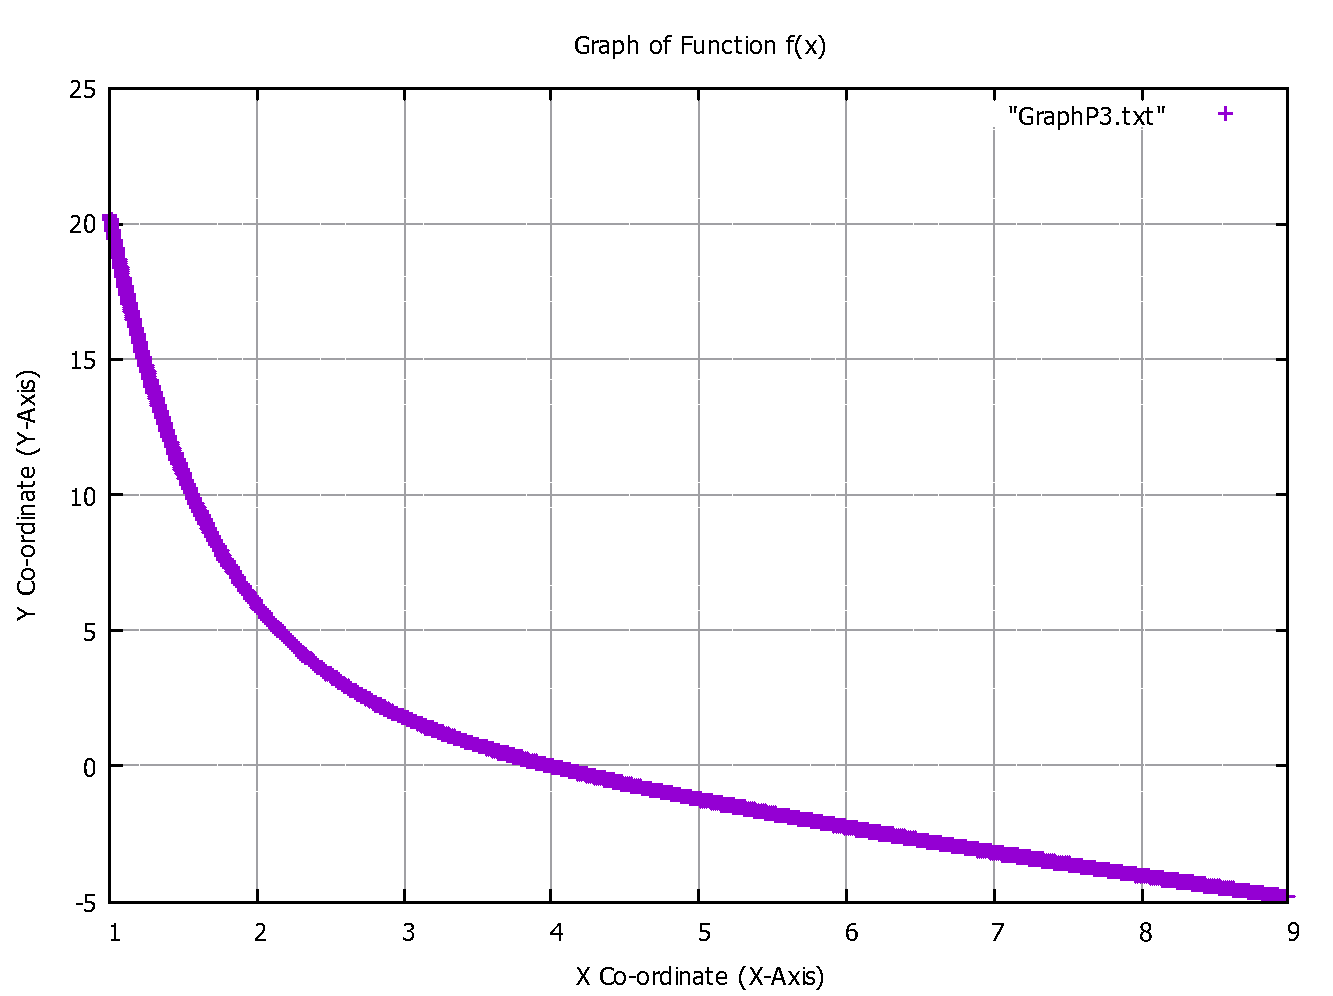
\includegraphics[width=\linewidth]{GraphP3.pdf}
    \caption{Graph of f(x)}
    \label{fig:5}
\end{figure}

Now I shall plot the graphs showing the error percentage as a function of the number of iterations considered while approximating the roots of $f(x)=0$ In Figure~\ref{fig:6}. The results are also summarized in Table~\ref{tab:tab3}.

\begin{figure}[!tbh]
  	\centering
  	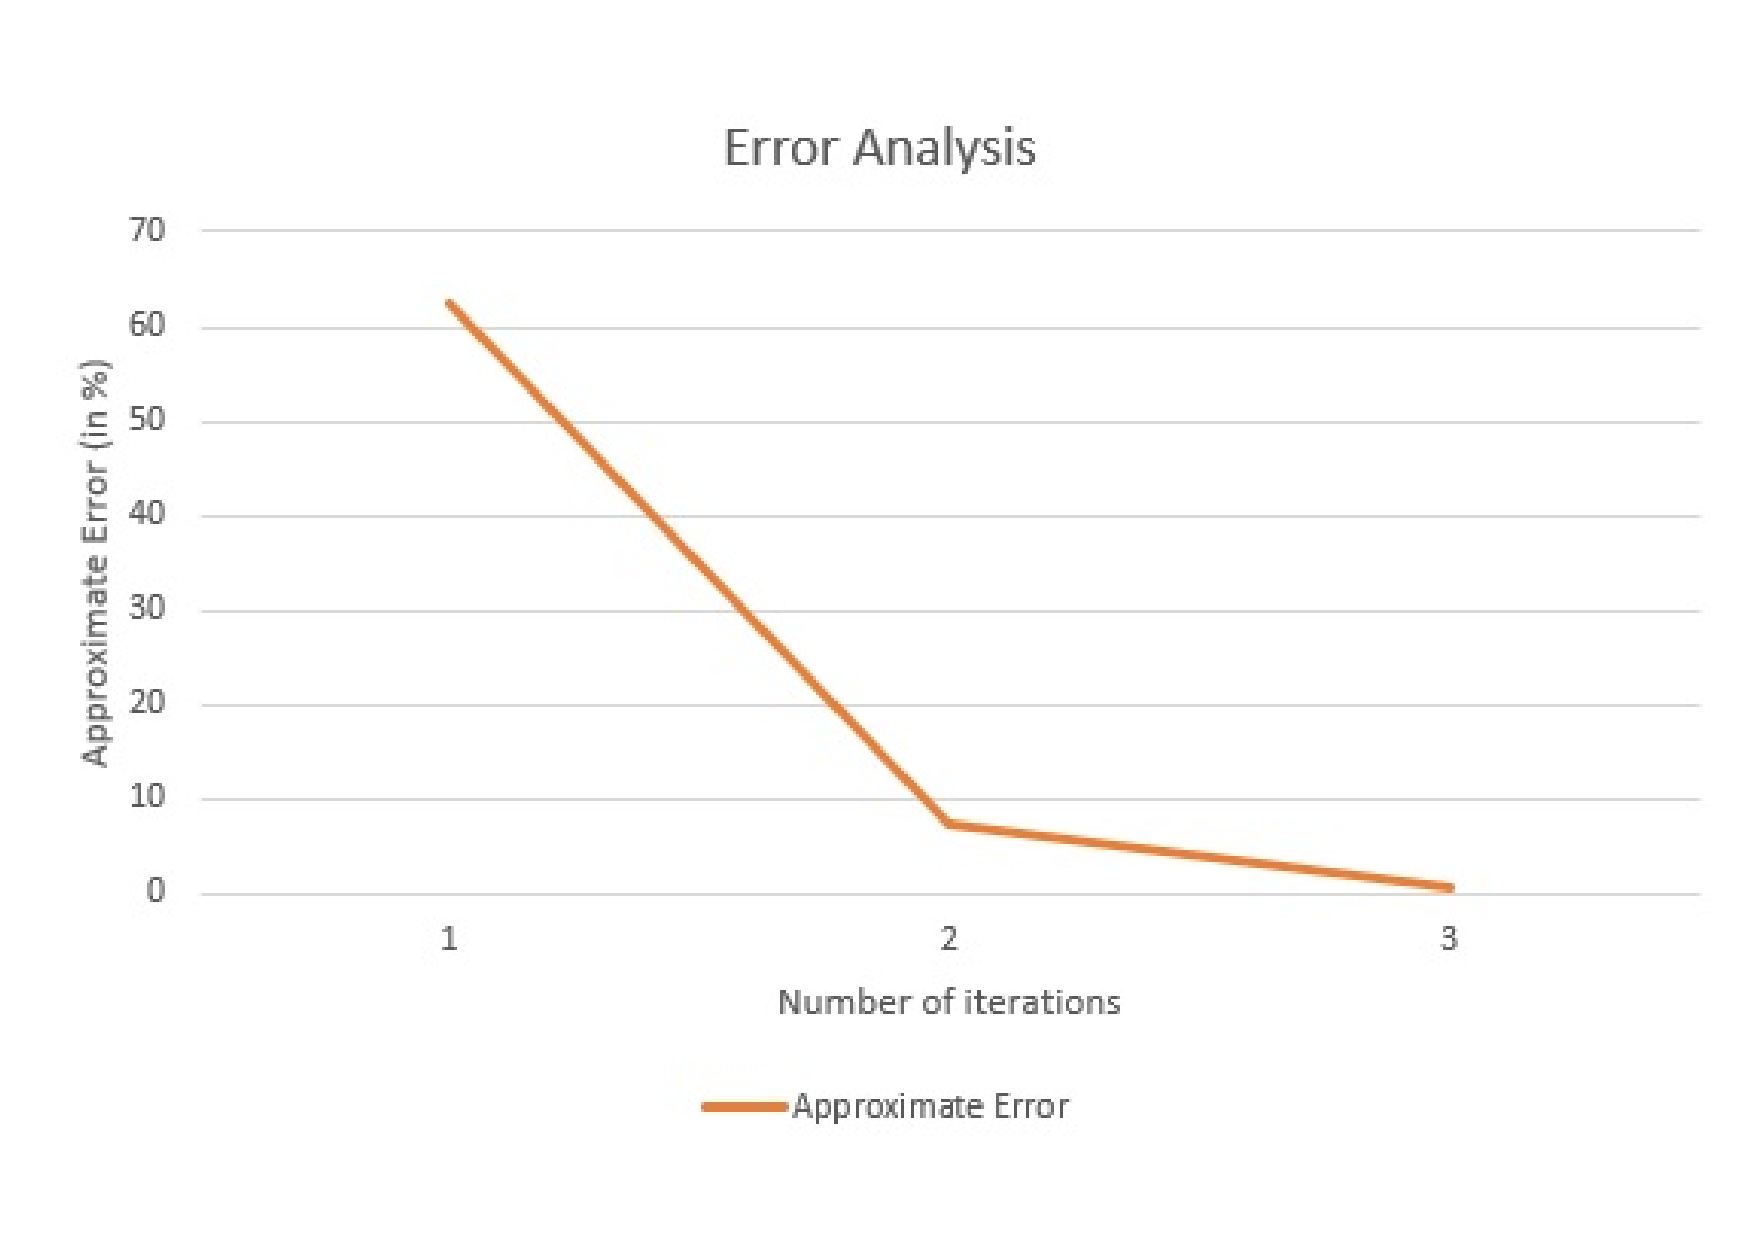
\includegraphics[width=0.9\textwidth]{Error-Analysis.pdf}
  	\caption{Approximate Error vs number of iterations considered while approximating the roots of $f(x)=0$.}
  	\label{fig:6} 
\end{figure}
\begin{figure}[!tbh]
  	\centering
  	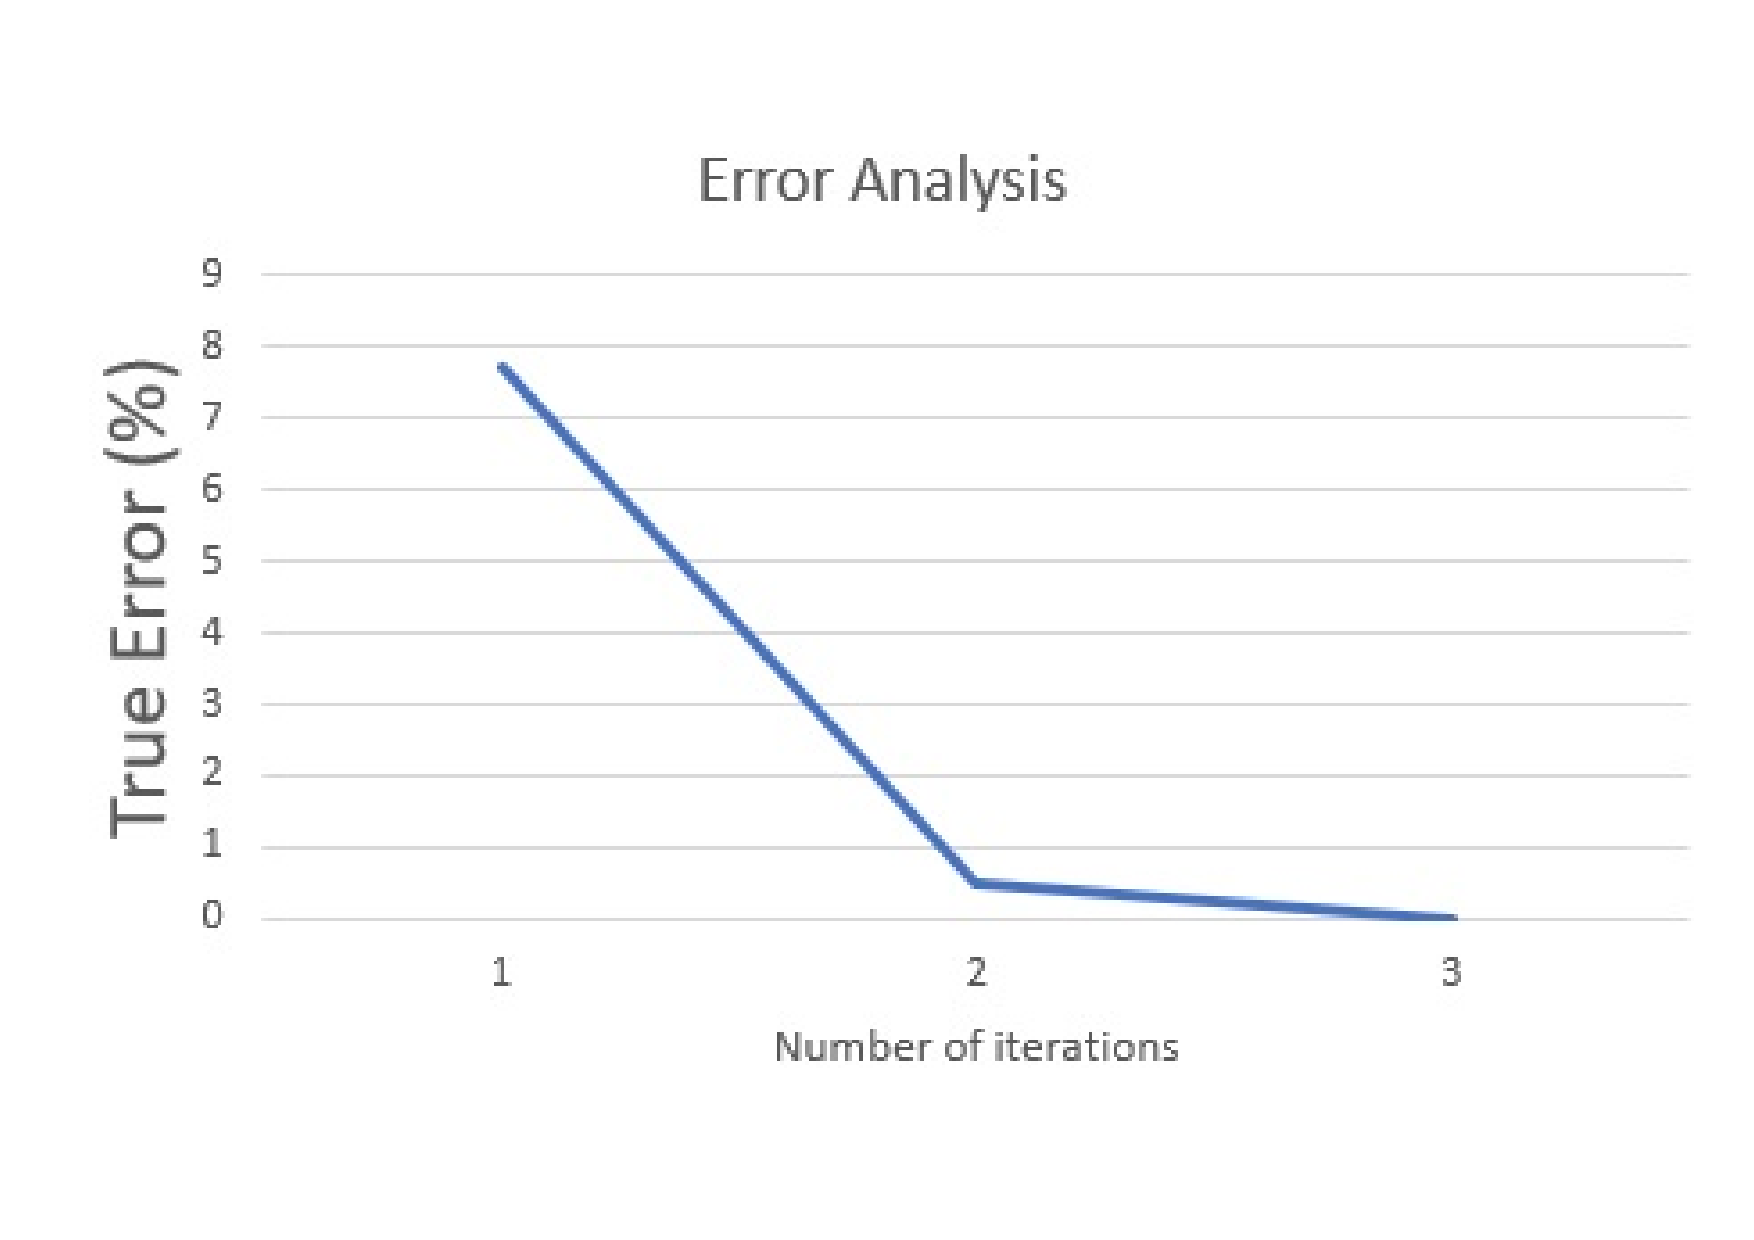
\includegraphics[width=0.9\textwidth]{TE3.pdf}
  	\caption{True Error vs number of iterations considered while approximating the roots of $f(x)=0$.}
  	\label{fig:86} 
\end{figure}
\begin{table}[!htb]
    \caption{Error percentage vs number of iterations}
    \centering
    \begin{tabular}{ccc}
    \toprule
    \textbf{$n$}& \textbf{Approximate Error} & \textbf{True Error}\\
    \midrule
         1 & 62.453196 & 7.702632\\
         2 & 7.245913 & 0.492398\\
         3 & 0.491483 & 0.000919\\
    \bottomrule 
    \end{tabular}
    \label{tab:tab3}
\end{table}

%%%%%%%%%%%%%%%%%%%%%%%%%%%%%%%%%%%%%%%%%%%%%%%%%%%%%%

\subsection{Inferences}
I deduce the following inferences from this problem:
\begin{itemize}
    \item [1] The sharp decline in the error percentage, as a function of $n$, the number of iterations. The approximate error percentage reaches a staggering 0.49\% and true error of 0.07\% after just three iterations.
    \item [2] It is quite obvious to conclude that the Newton-Raphson Method is one of the fastest converging root finding techniques. As compared to other root finding algorithms, Newton Raphson Method computes the result with desired efficiency in very less number of iterations generally , thus making it one of the fastest root finding algorithms. 
\end{itemize}

%%%%%%%%%%%%%%%%%%%%%%%%%%%%%%%%%%%%%%%%%%%%%%%%%%%%%%

\subsection{Code}
The code used for the experiments is mentioned in Listing~\ref{listing:4}. 

\inputminted[breaklines,
 mathescape,
 linenos,
 numbersep=5pt,
 frame=single,
 numbersep=5pt,
 xleftmargin=0pt]{c}{Newton.c}
 \captionof{listing}{Code snippet used in the problem.}
\label{listing:4}

%%%%%%%%%%%%%%%%%%%%%%%%%%%%%%%%%%%%%%%%%%%%%%%%%%%%%%

\subsection{Contributions}
In the above problem, \textit{my original contributions} are - 
\begin{itemize}
    \item Designing of the Algorithm and Code
    \item Plotting of the graph on GNU Plot and MS Excel
    \item Analysis of True Error and Approximate Error
    \item Tabulation of Results and Errors
    \item Drawing conclusions by looking at the Result obtained and Error Analysis.
\end{itemize}

\subsection{Alternate Methods}
We evidently see that the Newton Raphson Method is a fast and effective convergent root finding algorithm for functions having a single root as compared to Bisection and False Position Algorithms.

Howsoever, the Newton Raphson method is not suitable generally for functions having more than one root or a large part of their curve horizontal as they fail to converge in a short number of iterations.
%%%%%%%%%%%%% END OF QUESTION 1 %%%%%%%%%%%%%%%%%%%%
\newpage
\section{Problem 4}
Figure 1 shows a circuit with a resistor, an inductor, and a capacitor in parallel. Kirchhoff’s rules can be used to express the impedance of the system as \\
\begin{center}
     $ \frac{1}{Z} = (\frac{1}{R^2} + (\omega C-\frac{1}{\omega L})^2)^{\frac{1}{2}} $ \\
\end{center}
where Z = impedance ($\Omega$) and $\omega$ = the angular frequency. Find the $\omega$ that results in an impedance of 75 $\Omega$ using both bisection and false position with initial guesses of 1 and 1000 for the following parameters: R = 225 $\Omega$ , C = $6 * 10^{−7}$ F, and L = 0.5 H. Determine how many iterations of each technique are necessary to determine the answer to $e_a$ = 0.1 \%. Use the graphical approach to explain any difficulties that arise.
\begin{figure}[ht]
  \centering
  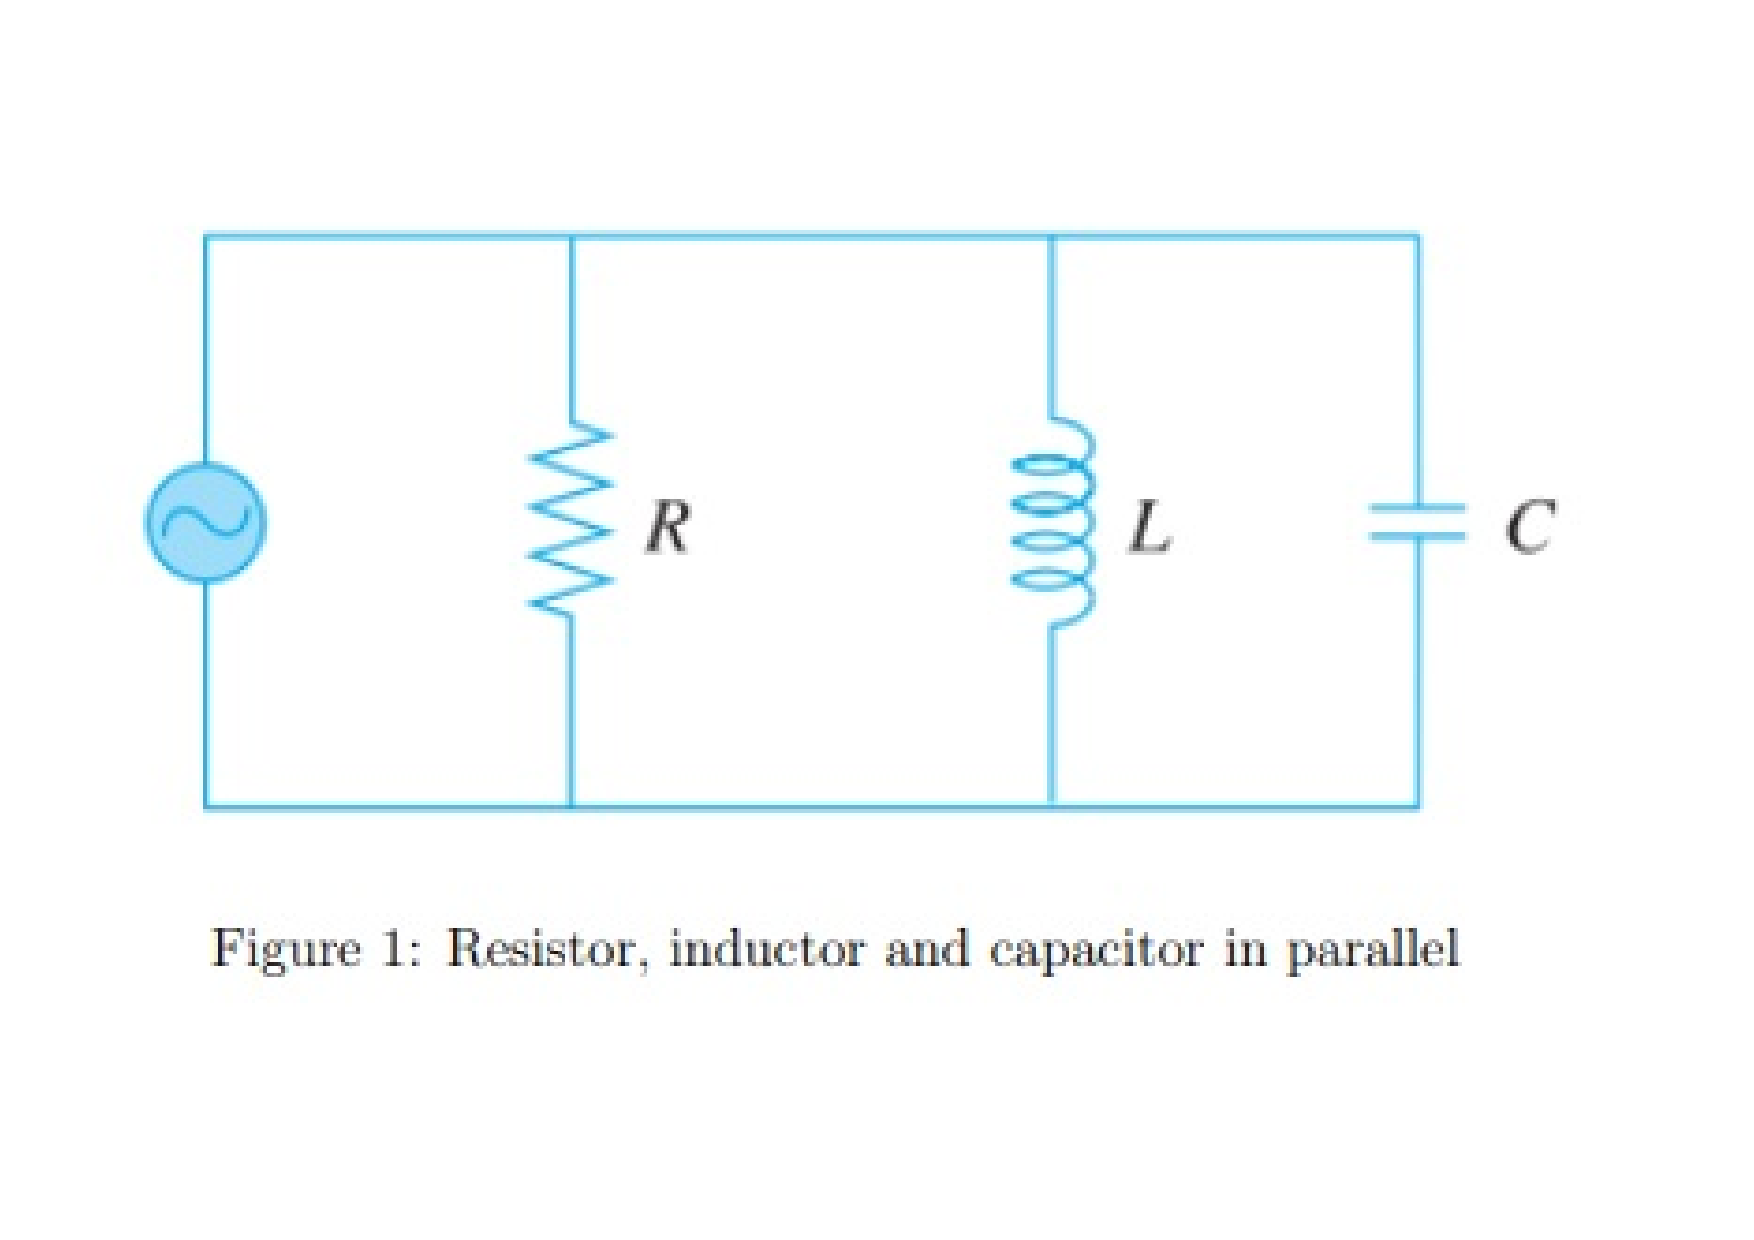
\includegraphics[width=\linewidth]{Question.pdf}
  \caption{Parallel Circuit}
  \label{fig:fig7a}
\end{figure}

\subsection{Approach}

We solve the problem by considering a function $f(x)$ that is equal to 
\begin{align}
    f(x) = (\frac{1}{R^2} + (xC-\frac{1}{xL})^2)^{\frac{1}{2}} - \frac{1}{Z}
\end{align}

We then use the Bisection Method and the False Position Method to find the roots of the equation $f(x)=0$

%%%%%%%%%%%%%%%%%%%%%%%%%%%%%%%%%%%%%%%%%%%%%%%%%%%%%%

\subsection{Algorithm}
In this section, I present the pseudocode/flowchart of the algorithm used to solve the problem.

Example: The pseudocode for finding the roots of f(x)=0 is provided in Algorithm~\ref{alg5} and Algorithm~\ref{alg6}
\begin{center}
\begin{algorithm}[H]\label{alg5}

\SetAlgoLined

Input $x_l,x_u,x_r$ \\
count = 1 \\
\While{$e_a$>e}{ 
$x_{rold} \gets x_r$ \;
$x_r \gets (x_l+x_u)/2$ \;
count++ \;
\If{$x_{r}$ \neq 0}{
$e_a \gets \frac{|x_r-x_{rold}|}{|x_r|} * 100$ \;
}
\If {f($x_l$)f($x_r$)=0} {
$e_a$=0\;
break \;
}
\If {f($x_l$)f($x_r$)<0} {
  $x_u\gets x_r$ \;
}
\Else {  
$x_l\gets x_r$ \;
}
}
return $x_r$ \\
 \caption{Approximating roots of $f(x)=0$ using Bisection Method}
\end{algorithm} 
\begin{algorithm}[H]\label{alg6}

\SetAlgoLined

Input $x_l,x_u,x_r$ \\
count = 1 \\
\While{$e_a$>e}{ 
$x_{rold} \gets x_r$ \;
$x_r \gets x_u - \frac{f(x_u)(x_l-x_u)}{f(x_l)-f(x_u)}$ \;
count++ \;
\If{$x_{r}$ \neq 0}{
$e_a \gets \frac{|x_r-x_{rold}|}{|x_r|} * 100$ \;
}
\If {f($x_l$)f($x_r$)=0} {
$e_a$=0\;
break \;
}
\If {f($x_l$)f($x_r$)<0} {
  $x_u\gets x_r$ \;
}
\Else {  
$x_l\gets x_r$ \;
}
}
return $x_r$ \\
\caption{Approximating roots of $f(x)=0$ using False Position Method}
\end{algorithm}    
\end{center}

%%%%%%%%%%%%%%%%%%%%%%%%%%%%%%%%%%%%%%%%%%%%%%%%%%%%%%
\subsection{Results}

Using Bisection Method, we find that the root is $x=157.947388$ with an approximate error of 0.077208 \% and true error of 0.000008\% after 13 iterations.\\

Using False Position Method, we get the root as  $x=189.4316$ with an approximate error percentage of 0.099767\% though the true error is around 20\% after 578 iterations. To get an answer near the actual root as indicated by Bisection Method or the Graphical Analysis, we need 1374 iterations in which the value of $x=158.1697$ and true error is roughly 0.5 \%. \\

In this section, I plot the graph of the function f(x) in the range [1,1000] using GNU plot in Figure~\ref{fig:Graph4} \\

\begin{figure}
\begin{subfigure}{.5\textwidth}
  \centering
  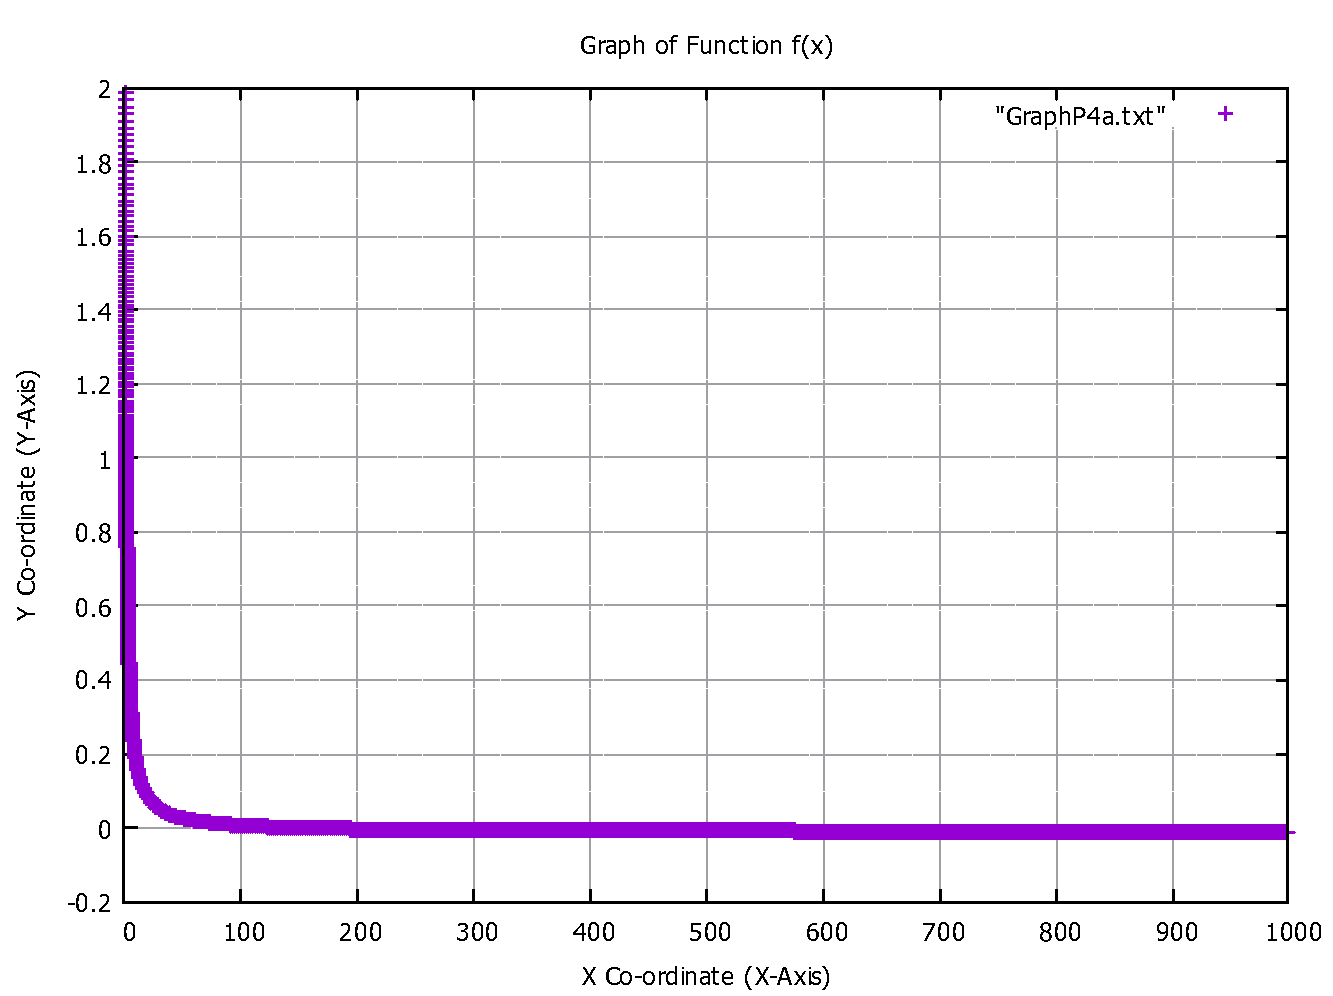
\includegraphics[width=\linewidth]{GraphP4a.pdf}
  \caption{Graph of f(x) plotted using Bisection Method CODE}
  \label{fig:fig8a}
\end{subfigure}
\begin{subfigure}{.5\textwidth}
  \centering
  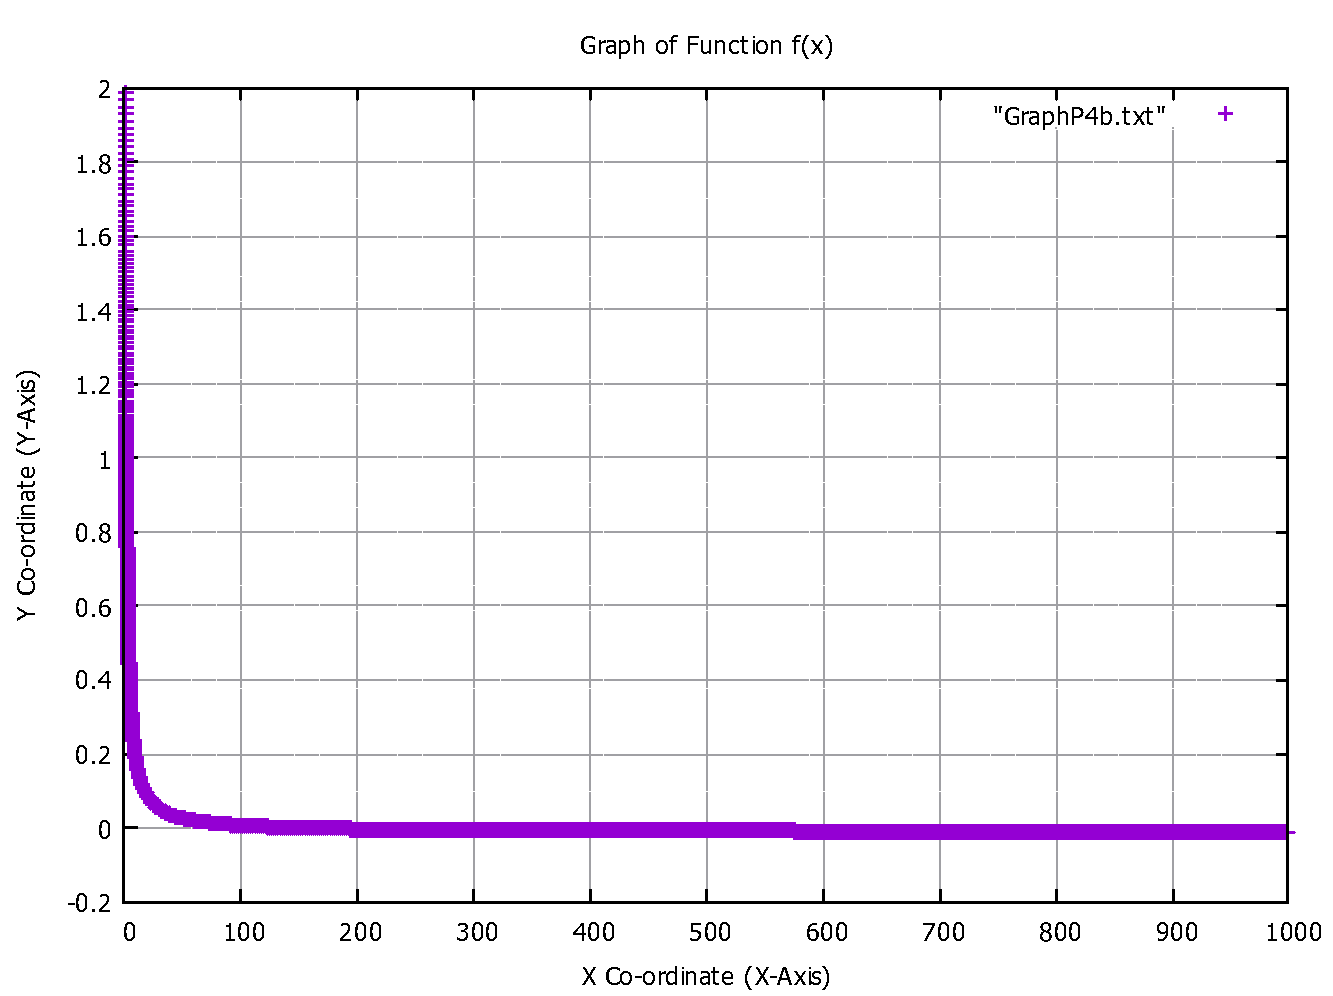
\includegraphics[width=\linewidth]{GraphP4b.pdf}
  \caption{Graph of f(x) plotted using False Position CODE}
  \label{fig:fig8b}
\end{subfigure}
\caption{Graph of f(x)}
\label{fig:Graph4}
\end{figure}

Now I shall plot the graphs showing the error percentage as a function of the number of iterations considered while approximating the roots of $f(x)=0$ In Figure~\ref{fig:fig9a} and~\ref{fig:fig9b}. The results are also summarized in Table~\ref{tab:tab6} and in Table~\ref{tab:tab86}.

\begin{figure}[ht]
\begin{subfigure}{.5\textwidth}
  \centering
  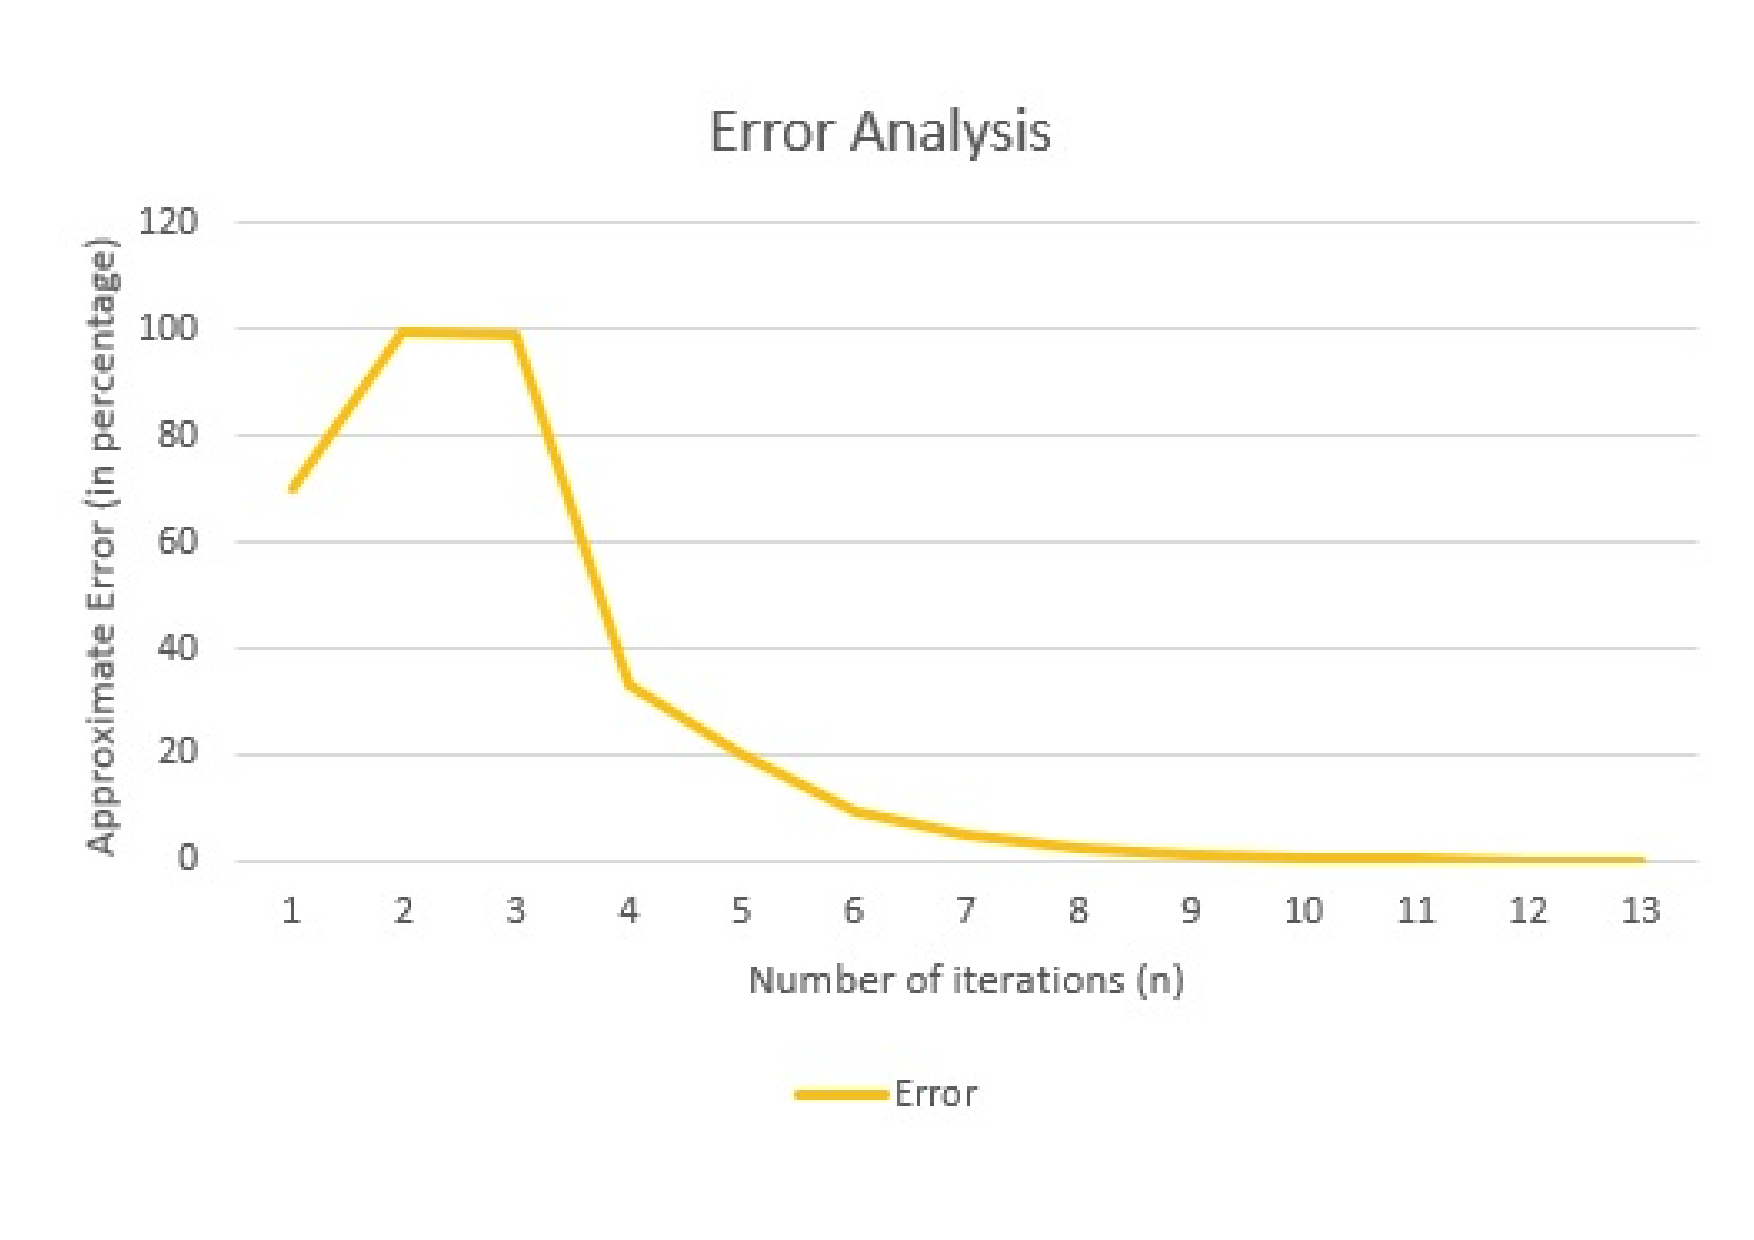
\includegraphics[width=\linewidth]{Error4a.pdf}
  \caption{Error vs No. of iterations for Bisection Method}
  \label{fig:fig9a}
\end{subfigure}
\begin{subfigure}{.5\textwidth}
  \centering
  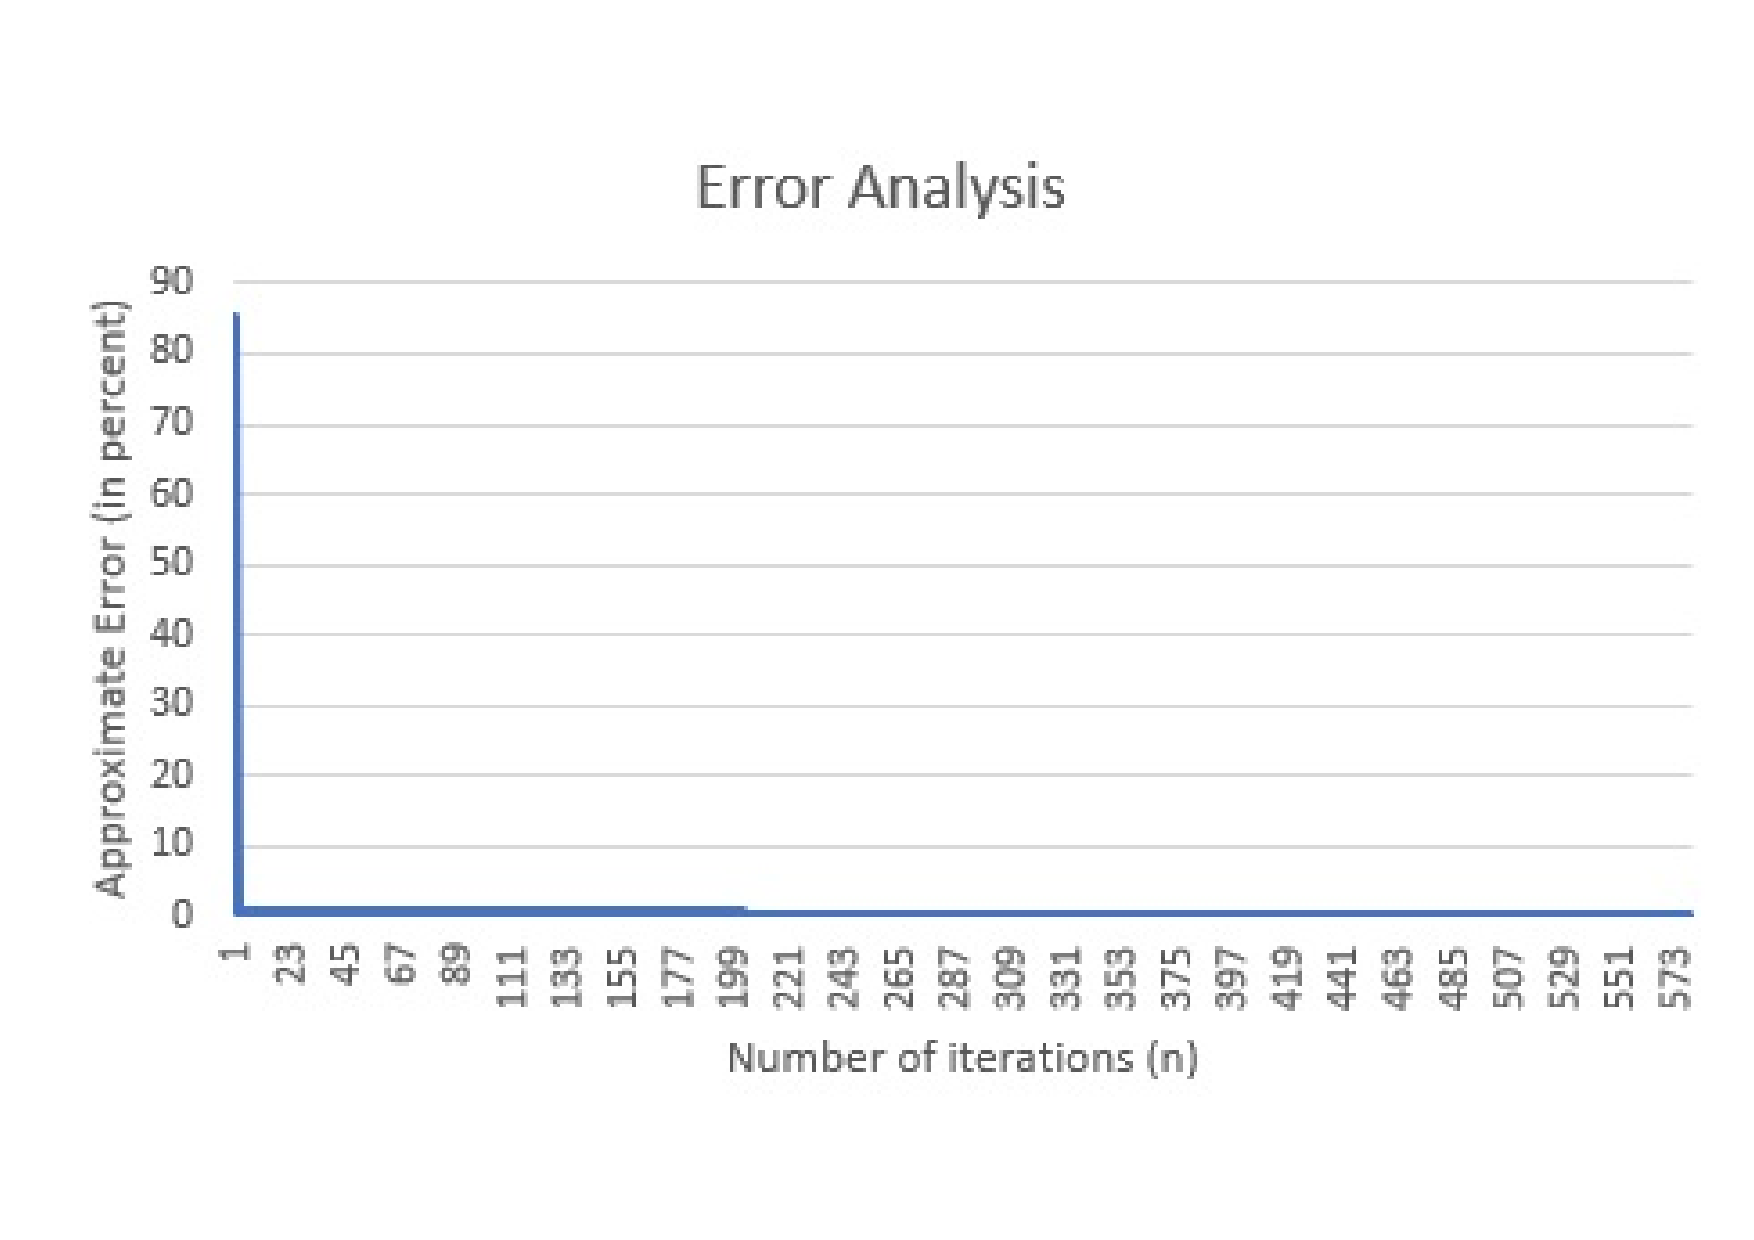
\includegraphics[width=\linewidth]{Approx.pdf}
  \caption{Error vs No. of iterations for False Position Method}
  \label{fig:fig9b}
\end{subfigure}
\caption{Approximate Error (in percent) vs Number of iterations considered while approximating the roots of $f(x)=0$.}
\label{fig:q4}
\end{figure}
\begin{figure}[ht]
\begin{subfigure}{.5\textwidth}
  \centering
  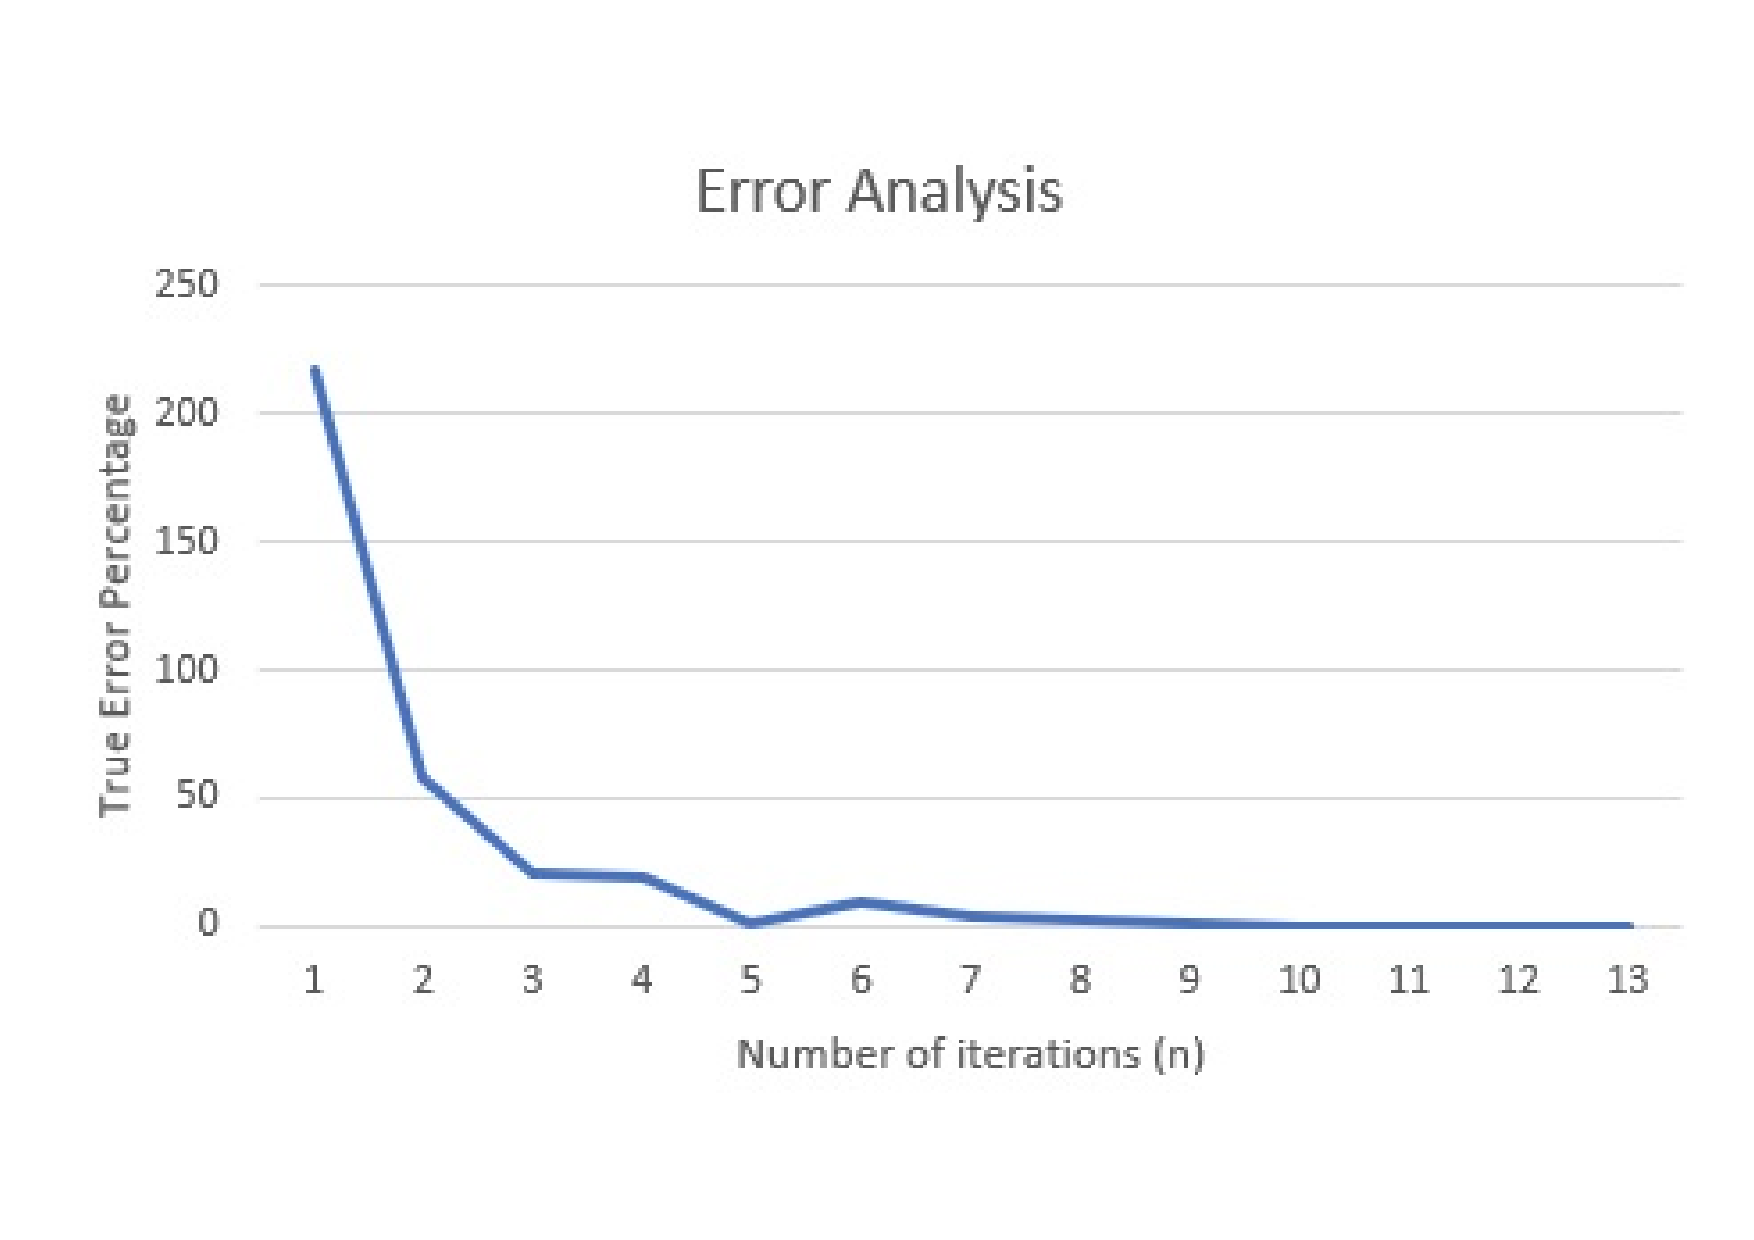
\includegraphics[width=\linewidth]{TE4a.pdf}
  \caption{Error vs No. of iterations for Bisection Method}
  \label{fig:fig89a}
\end{subfigure}
\begin{subfigure}{.5\textwidth}
  \centering
  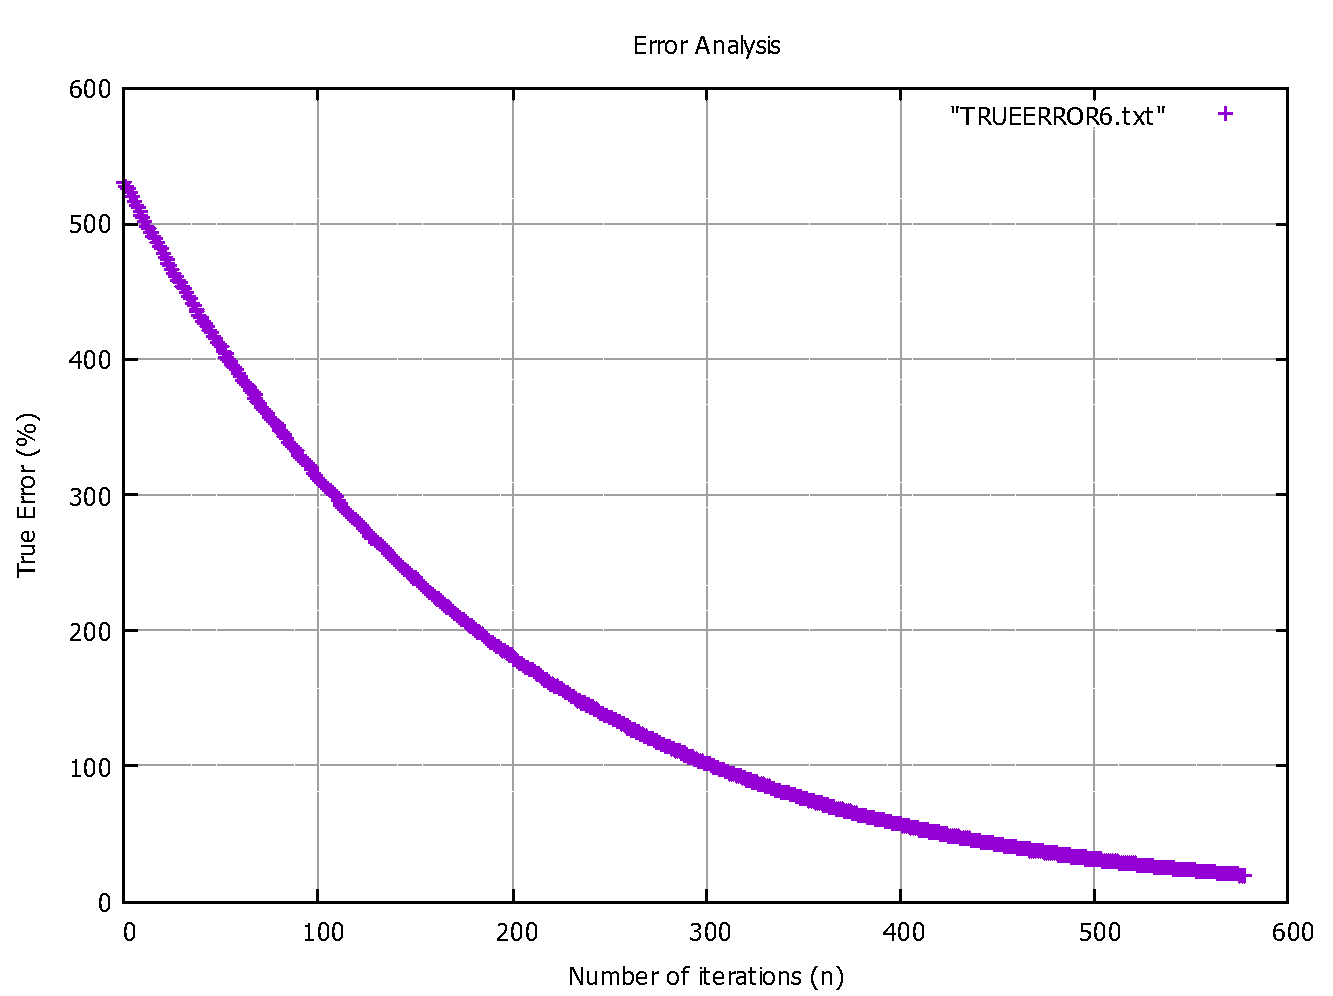
\includegraphics[width=\linewidth]{TE4b.pdf}
  \caption{Error vs No. of iterations for False Position Method}
  \label{fig:fig89b}
\end{subfigure}
\caption{True Error (in percent) vs Number of iterations considered while approximating the roots of $f(x)=0$.}
\label{fig:q84}
\end{figure}

\begin{table}[!htb]
    \caption{Error percentage vs number of iterations for Bisection Method($n$)}
    \centering
    \begin{tabular}{ccc}
    \toprule
    \textbf{$n$}& \textbf{Approximate Error} &\textbf{True Error} \\
    \midrule
          1 & 70.029970 & 216.877644 \\
          2 & 99.601196 & 58.755383\\
          3 & 99.205561 & 20.305747\\
          4 & 33.156323 & 19.224818\\
          5 & 19.872687 & 0.540465\\
          6 & 9.038270 & 9.342177\\
          7 & 4.733027 & 4.400856\\
          8 & 2.423875 & 1.930196\\
          9 & 1.226806 & 0.694865\\
         10 & 0.617189 & 0.077200\\
         11 & 0.309550 & 0.231632\\ 
         12 & 0.154536 & 0.077216\\
         13 & 0.077208 & 0.000008\\
    \bottomrule
    \end{tabular}
    \label{tab:tab6}
\end{table}

\begin{table}[!htb]
    \caption{Error percentage vs number of iterations for False Position Method($n$)}
    \centering
    \begin{tabular}{ccc}
    \toprule
    \textbf{$n$}& \textbf{True Error} & \textbf{Approximate  Error}\\
    \midrule
          10 & 506.207816 & 0.434530 \\
          50 & 410.560611 & 0.425626 \\
          100 & 314.418342 & 0.410085 \\
          200 & 181.429054 & 0.361988 \\
          500 & 31.750415 & 0.143787 \\
          578 & 19.933358 & 0.099767 \\
    \bottomrule
    \end{tabular}
    \label{tab:tab86}
\end{table}

%%%%%%%%%%%%%%%%%%%%%%%%%%%%%%%%%%%%%%%%%%%%%%%%%%%%%%

\subsection{Inferences}
I deduce the following inferences from this problem:
\begin{itemize}
    \item [1] The sharp decline in the error percentage, as a function of $n$ in Figure~\ref{fig:fig9a} and Figure~\ref{fig:fig9b} shows that the approximate error decreases as the number of iterations increases. 
    \item [2] However, we see that the Bisection Method gives a better efficiency in limited number of iterations as compared to the False Position Method, contrary to the general trend observed. 
    \item [3] We also deduce that the Bisection Method converges faster than the False Position Method in this problem.
    \item [4] We clearly see that the False Position gives an answer of around x=189.431620 after 578 iterations with an approximate error of less than 0.1\% but with a higher true error of around 20\%.
    \item [5] This is because of the near flat nature of the graph, that the False Position Method fails. 
    \item [6] This makes us realise that the Bisection Method gives a reliable result though slow, and the False position Method is not accountable in spite of its rapid convergence.  
    \item [7] We clearly see that the true error goes beyond 100 \% in some of the iterations. This can be explained in the following manner - The root $x_r$ is much greater than {$x_{root}$} thus, the ratio of their difference to the root exceeds 1. Thus, the error percentage goes beyond 100\%.
    \item [8] False Position Method is ill suited for graphs having a large horizontal portion as evident.
\end{itemize}

%%%%%%%%%%%%%%%%%%%%%%%%%%%%%%%%%%%%%%%%%%%%%%%%%%%%%%

\subsection{Code}
The code used for the problem is mentioned in Listing~\ref{listing:8} and Listing~\ref{listing:9}. 

\begin {itemize}
\item [(1)] Bisection Method CODE
\end {itemize}
\inputminted[breaklines,
 mathescape,
 linenos,
 numbersep=5pt,
 frame=single,
 numbersep=5pt,
 xleftmargin=0pt]{c}{Bisection2.c}
 \captionof{listing}{Code snippet used in the problem.}
\label{listing:8}

\begin {itemize}
\item [(2)] False Position Method CODE
\end {itemize}
\inputminted[breaklines,
 mathescape,
 linenos,
 numbersep=5pt,
 frame=single,
 numbersep=5pt,
 xleftmargin=0pt]{c}{FalsePosition2.c}
 \captionof{listing}{Code snippet used in the problem.}
\label{listing:9}

%%%%%%%%%%%%%%%%%%%%%%%%%%%%%%%%%%%%%%%%%%%%%%%%%%%%%%

\subsection{Contributions}
In the above problem, \textit{my original contributions} are - 
\begin{itemize}
    \item Designing of the Algorithm and Code
    \item Plotting of the graph on GNU Plot and MS Excel
    \item Analysis of True Error and Approximate Errors
    \item Drawing conclusions and inferences by looking at the Result obtained and Error Analysis.
\end{itemize}


%%%%%%%%%%%%%%%%%%%%%%%%%%%%%%%%%%%%%%%%%%%%%%%%%%%%%%

\subsection{Alternate Methods}
\begin{itemize}
\item [1] We can clearly conclude that since a large part of the graph is horizontal, the slope is near to zero. Thus the methods involving slope in the denominator converge very slowly and a large number of iterations. Thus, the False Position and the Newton Raphson Method fail to converge quickly in comparison to the Bisection Method. Thus, the Bisection Method serves as a good Numerical Method to use for this particular question. \\
\item [2] We need to do suitable modifications to thus correct the pitfalls of the False Position and Newton Raphson Method in case of functions having a large horizontal portion. \\
\item [3] In addition, we also need to tackle the situation of multiple roots and tangential roots, which cannot be easily detected by the Bisection Algorithm or the False Position Algorithm in its present form and needs suitable modifications. \\
\end{itemize}

\end{document}
